\documentclass[12pt]{article}
\usepackage{amsmath}
\usepackage{amsfonts}
\usepackage{amssymb}
\usepackage{graphicx}
\usepackage{caption}
\usepackage{math tools}
\usepackage{lipsum}
\usepackage{stackengine}
\usepackage{fancyhdr}
\usepackage{caption}
\usepackage{tikz}
\usetikzlibrary{shapes.geometric, arrows}
\usepackage{float}
\usepackage[a4paper,left=1in,right=1in,top=1in,bottom=1in,footskip=.25in]{geometry}
\usepackage{etoolbox}
\usepackage[nottoc]{tocbibind}
\usepackage{tabu}
\usepackage{enumitem,kantlipsum}
\usepackage{appendix}
\usepackage{pdfpages}
\usepackage{geometry}
\usepackage{color,colortbl}
\usepackage{hyperref}
\begin{document}

	\begin{titlepage}
		\centering
		
		\begin{figure}
			\begin{center}
				
\includegraphics[scale=.2]{tubaf.pdf}  
			\end{center}
			
		\end{figure}
		
		
		
		%\includegraphics[width=0.15\textwidth]{download}\par\vspace{1cm}
		{\scshape \LARGE \textbf{Technische Universit\"at Bergakademie Freiberg} \par}
		\vspace{1cm}
		{\scshape\Large PERSONAL PROGRAMMING PROJECT\par}
		{\scshape\Large (PPP)\par}
		\vspace{1.5cm}
		{\huge\bfseries Implementation of Gradient Elasticity Model In FEM \par}
		\vspace{2cm}
		{\scshape\Large \textbf{Dhaval Rasheshkumar Patel}\par}
		{\scshape\Large 63940\par}
		\vfill
		{\normalsize\ Supervised by\par}
		
		Dr.~ \textsc{Sergii Kozinov}
		
		\vfill
		
		% Bottom of the page
		{\large \today\par}
	\end{titlepage}
	\clearpage
    \textbf{\LARGE Abstract}\\
    \\
    { \large During this "Personal Programming Project(PPP)", the "Strain Gradient Elasticity Theory" is implemented through the FEM model. Within this, the element QU34L4, developed by Shu et al. is integrated as user defined element via the commercial software ABAQUS. The mixed type of FEM formulation developed by John Y. \cite{shu1999finite} is used for this theory.
    In this PPP, the User Element routine(UEL) for QU34L4 element and User Material routine(UMAT) for two different strain gradient material (\cite{amanatidou2002mixed},\cite{shu1999finite}) are formulated for 2D case. The numerical results of Plate-720 model is analysed for this theory. Two different patch test is also done to compare the numerical results obtain from this UEL with analytical solutions. Programming was done completely by myself without any external help. I have started with literature sources \cite{amanatidou2002mixed} and \cite{shu1999finite} and decided to follow the derivations by Shu et al \cite{shu1999finite}. Later on I got an access to the pdf of Diploma Thesis of Mr. L. Zybell [8], however without any code (or part of the code) or scripts. As an extra task, an attempt to extend this UEL for 3D model is also done.}





    \newpage
    	\listoffigures
    	\listoftables
    \clearpage
    \tableofcontents
    \clearpage

\section{Introduction}
Classical continuum solid mechanics theories, such as linear or non-linear elasticity and plasticity, have been used in wide range of fundamental problems and applications in various fields, but "Classical Continuum Constitutive Models" possess no material/intrinsic scale. So in this regime of micron and nano-scales that experimental evidence and observations have suggested that classical continuum theories do not suffice for an accurate and detailed description in the modelling of size dependent phenomena. Moreover, classical elastic singularities as those emerging during the application of point loads and description of size effects also not solve by it.
\newline
\par
In General, in Gradient elasticity theories, the length scales enter the constitutive equations through the elastic strain energy function, which, in this case depends not only on the strain tensor but also on gradients of the strain tensors. Gradient Elasticity theories provide extensions of the classical equations of elasticity with additional higher order spatial derivatives of strains and stresses, but in Gradient elasticity theory one of the most challenging task is to keep the number of additional constitutive parameters to a minimum.
\newline
\par
Stress equation of equilibrium, constitutive equations and boundary conditions of the "Strain Gradient theory" were first given in a non-linear form by Toupin in 1960s. After this famous Strain Gradient elasticity theory in three different forms proposed by Mindlin in 1960s. In such theories , when the problem is formulated in terms of displacements, the governing partial differential equation contains the fourth order derivative of displacements. If traditional finite element formulation are used for the numerical solution of such problems, then $C^{1}$ displacement continuity is required. $C^{1}$ displacement continuity means displacement and its first derivative is continuous in inter-element. However, in FEM there was no any robust $C^{1}$ continuous element. So an alternative mixed finite elements formulation is developed, in which both the displacement and the displacement gradients are used as independent unknowns and their relationship is enforced using Lagrange Multiplier Method. In 1999 JOHN Y. SHU proposed the mixed finite formulation based on Toupin—Mindlin theories, in which only $C^{0}$ continuous element was used. After this in 2002 E. Amanatidou and N. Aravas also proposed the Mixed type FEM formulation for Toupin—Mindlin theories and also used $C^{0}$ continuous element.
\newline  
\par
In the present "Personal Programming Project" report, in the very first section we discussed the theoretical background of the strain gradient elasticity theory with its evolutions and different versions. Following to this section, we discussed in brief few of them theories. After this the Mixed type of FEM formulation with $C^{0}$ continuous element for Strain Gradient theory is discussed in details. In the last, the results of this implemented FEM model is shown. In addition to this the results of the verification tests are also shown.
\newpage
 
\section{Theoretical Background}
In this Section the main focus is to understand the "Classical Strain Gradient Elasticity Theory" and motivation behind the evolution of Strain Gradient Elasticity theories. In this section the brief overview of Toupin's, Mindlin's, Eringen's and Aifantis theory is given. After this also discussed about different possible FEM formulation.  
     \begin{figure}[H]
     	\begin{center}
     	     	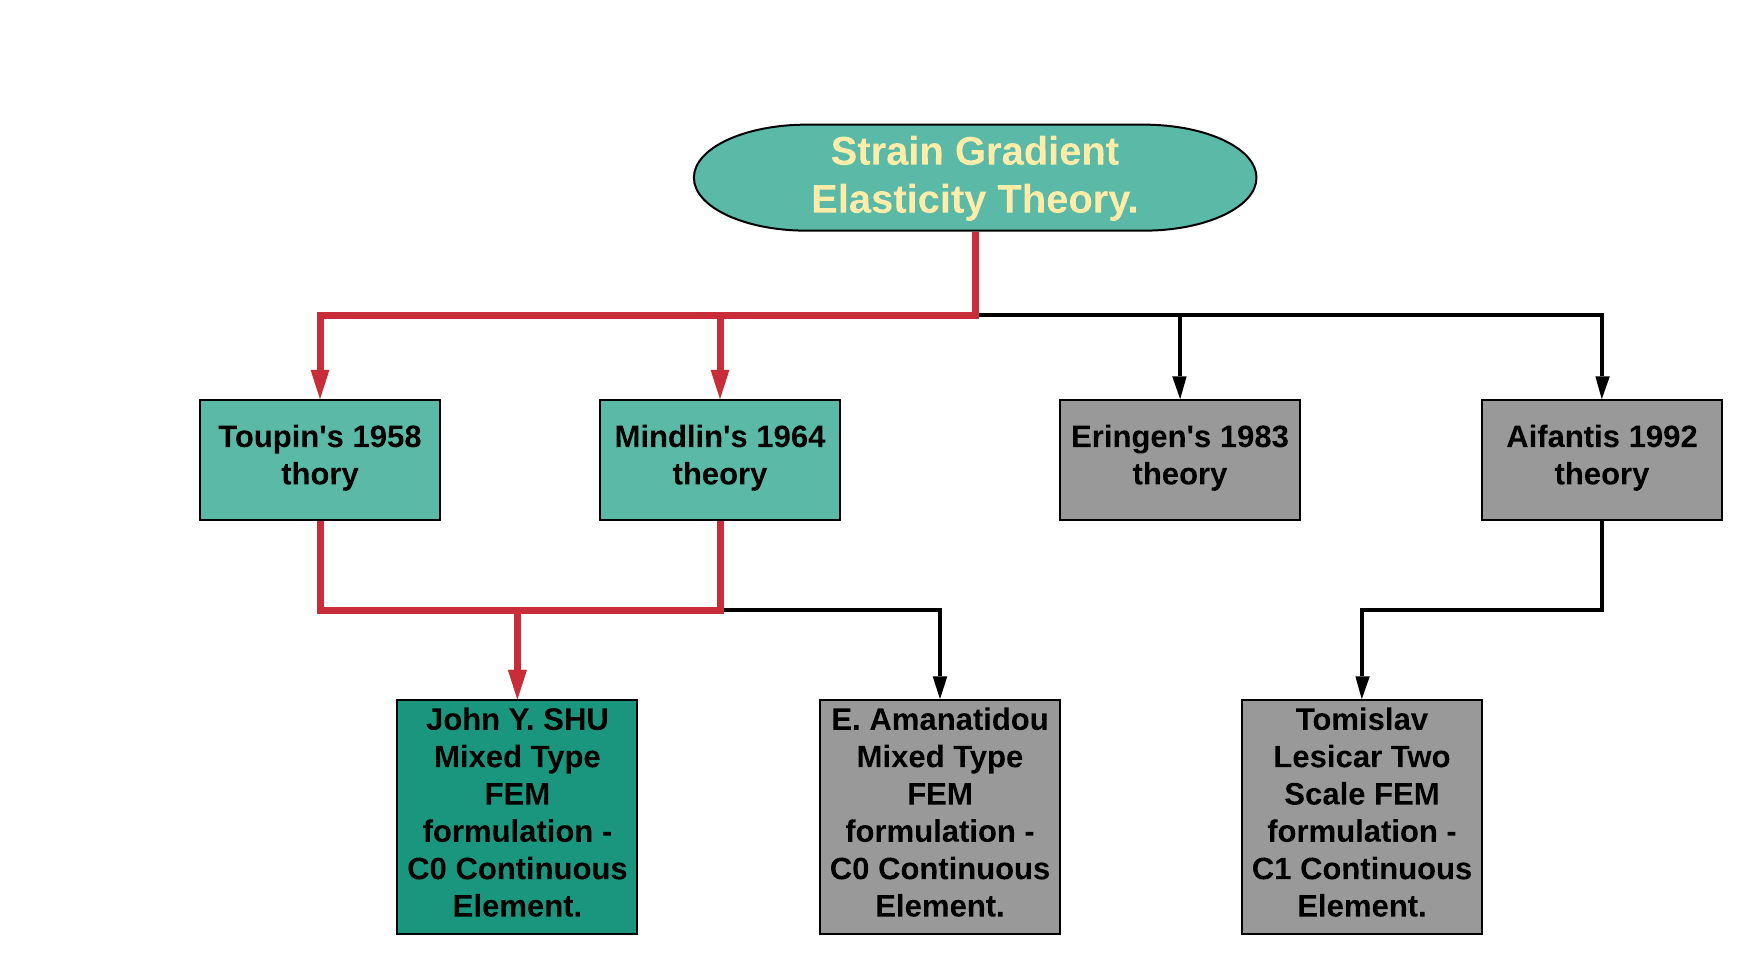
\includegraphics[scale=0.5]{straingradienthistory.png}
     	\end{center}
     	\caption{The history of Strain Gradient Theory}
     \end{figure}
\subsection{Mindlin's 1964 Theory.}
In the early 1960s, the Mindlin \cite{mindlin1968first} presented a theory of elasticity with Microstructure length, in which he distinguished between kinematic quantities on two scale micro and macro. As discussed in introduction that it is very challenging task to keep the number of constitutive parameters to a minimum. In this theory constitutive tensor contains 1764 coefficients in total, but for isotropic material its reduced drastically to amount 18. Mindlin present the Strain energy equation as,
\begin{equation}\label{first}
\begin{aligned}
U= &\frac{1}{2}\lambda\varepsilon_{ii}\varepsilon_{jj}+\mu\varepsilon_{ij}\varepsilon_{ij}+\frac{1}{2}b_1 \gamma_{ii} \gamma_{jj}+\frac{1}{2}b_2 \gamma_{ij} \gamma_{ij}+\frac{1}{2}b_3 \gamma_{ij} \gamma_{ji}+g_1\gamma_{ii}\varepsilon_{jj}
\\   
&+g_2(\gamma_{ij}+\gamma_{ji})\varepsilon_{jj}+a_1\kappa_{iik}\kappa_{kjj}+a_2\kappa_{iik}\kappa_{jkj}+\frac{1}{2}a_3\kappa_{iik}\kappa_{jjk}
\\
&+\frac{1}{2}a_4\kappa_{iij}\kappa_{ikk}
 +a_5\kappa_{iij}\kappa_{kik}
+\frac{1}{2}a_8\kappa_{iji}\kappa_{kjk}+\frac{1}{2}a_{10}\kappa_{ijk}\kappa_{ijk}
\\
&+a_{11}\kappa_{ijk}\kappa_{jki}+\frac{1}{2}a_{13}\kappa_{ijk}\kappa_{ikj}
+\frac{1}{2}a_{14}\kappa_{ijk}\kappa_{jik}
+\frac{1}{2}a_{15}\kappa_{ijk}\kappa_{kji}
\end{aligned}
\end{equation}  

where $\lambda$ and $\mu$ are the usual Lame constants and the various $a_i$ , $b_i$ and $g_i$ are 16 additional constitutive coefficients. However for practical purpose the use of eq(1) is very limited as it requires so much additional coefficients. In later 1960s Mindlin also formulated the simpler version of his own elasticity theory by making assumption of expressing the strain energy density in terms of displacement only. So in last he proposed three different form of it. However, the equation of strain energy density is of order four and it requires $C^{1}$ continuity.
\newpage

\subsection{Aifanti's 1992 Theory.} 
In the early 1990s, motivated by own work in plasticity and non-linear elasticity, Aifantis \cite{askes2011gradient} suggested to extend the linear constitutive model given by Mindlin in form II, in which second order terms are expressed as the strain gradient tensor. So he modified this Mindlin form II by neglecting the most of the gradient coefficients. Mindlin present that for a general isotropic elastic solid the strain energy density depends upon
$\varepsilon_{ij}$ and $\kappa_{ijk}$ as the following,
\begin{equation}\label{two}
\begin{aligned}
W(\varepsilon,\kappa) = 
& G(\varepsilon_{ij}\varepsilon_{ij}+\frac{\nu}{1-2\nu}\varepsilon_{ij}\varepsilon_{ij}) \\
&    +a_1\kappa_{iik}\kappa_{kjj}+a_2\kappa_{iik}\kappa_{kjj}+a_3\kappa_{iik}\kappa_{kjj}+a_4\kappa_{iik}\kappa_{kjj}+a_5\kappa_{iik}\kappa_{kjj}
\end{aligned}
\end{equation}
where G is elastic shear modulus, $\nu$ is Poisson's ratio and $a_1$,$a_2$,$a_3$,$a_4$,$a_5$ are material constants.   
\newline
In this he considered,
\newline
\begin{equation}
\begin{aligned}
& a_1 = a_3 = a_5 = 0,   &   a_2 = \frac{\nu}{1-2\nu}Gl^2, &&  a_4 = Gl^2
\end{aligned}
\end{equation} 
Accordingly, the strain energy density is defined as
\begin{equation}
W = \frac{1}{2}\lambda\varepsilon_{ii}\varepsilon_{jj}+\mu\varepsilon_{ij}\varepsilon_{ij}+l^2(\frac{1}{2}\lambda\varepsilon_{ii,k}\varepsilon_{jj,k}+\mu\varepsilon_{ij,k}\varepsilon_{ij,k})
\end{equation}
In Eq. (4), $\lambda$ and $\mu$ are Lame constants, while $l$ represents microstructural parameter (material length scale).However this equation(4) of strain energy also requires 
$C^{1}$ continuous element.
\newline
\newline
\textbf{Conclusion of above both theories (2.1) and (2.2) : }
\newline
\newline
In above both strain gradient theories the principle of virtual work for a linear elastic strain gradient solid can be expressed as
\begin{equation}
\int\limits_\upsilon\! [\sigma_{ij} \delta\varepsilon_{ij} + \tau_{ijk}\delta\eta_{ijk}]  dV = \int\limits_\upsilon\! [b_k\delta u_k] dV + \int\limits_s \! [f_k\delta u_k+r_kD\delta u_k]dS
\end{equation}
where $D(.) = n_k\frac{\partial(.)}{\partial x_k}$ is surface normal-gradient operator, $b_k$ is the body force per unit volume
of the body $V$ while $f_k$ and $r_k$ are the truncation and the double stress traction per unit area of the surface $S$. They are in equilibrium with the Cauchy stress $\sigma_{ij}$ and the higher-order stress $\tau_{ijk}$ according to
\begin{equation}
b_k + (\sigma_{ij}-\tau_{jik,j})_{,i} = 0
\end{equation}
The constitutive law governing the stress $\sigma_{ij}$ and the higher-order stress $\tau_{ijk}$ for an elastic solid is derived through $\sigma_{ij} = \partial w / \partial \varepsilon_{ij}$ and $\tau_{ijk}= \partial w / \partial \eta_{ijk}$ where w is the strain energy density per unit volume. In this Cauchy stress $\sigma_{ij}$ is work conjugate to the strain $\varepsilon_{ij}$ and higher-order stress $\tau_{ijk}$ is work conjugate to the strain gradient  $\eta_{ijk}$.
\newline
\newline
Here, second-order derivatives of displacement occurred in the principle of virtual work Eq.(5), implying that displacement-based elements of $C^1$-continuity are indispensable in a finite element formulation. However there were no robust $C^1$ continuous elements available at that time for the application of fem formulation of above mentioned both strain gradient theories.

\section{Different FEM Approach}
There are different FEM approach to the Strain Gradient Elasticity theories are available because of the fact that $C^1$ continuous elements are very difficult to formulate and on the other hand there are also a mixed finite element formulation of strain gradient elasticity derived, which only requires $C^0$ continuity.

\subsection{Tomislav Lesicar - Two scale FEM formulation} 
\subsubsection{ C1-Continuous Element}
The Aifantis strain gradient theory given in subsection (2.2) has been embedded into finite element framework by Tomislav Lesicar, Zdenko Tonkovic and Jurica Soric \cite{lesivcar2017two}. They used the three node triangular finite element named C1PE3 \cite{putar2017damage}. The element is shown in
Fig 2. \cite{putar2017damage}. It contains twelve degrees of freedom (DOF) per node, and it satisfies $C^1$ continuity with assumptions of the plane strains with unit thickness.
\newline
     \begin{figure}[H]
     	\begin{center}
	      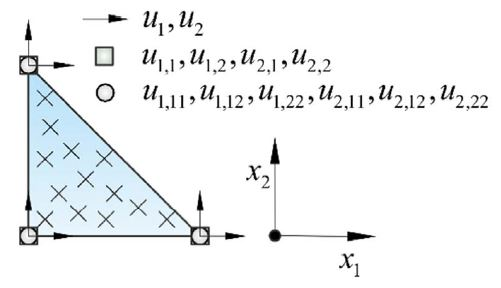
\includegraphics[scale=0.8]{Tri_Element.JPG}  
	    \end{center}  
        \caption{C1-Continuous Triangular Element \cite{putar2017damage}}
     \end{figure}
\subsubsection{ Higher-order stress and strain gradient tensor} 
They used the same weak form of the finite element formulation as given by Eq.(5). Furthermore, using the basic finite element relations strain and stress tensors can be expressed as
\begin{equation}
\varepsilon = Bu,      \sigma=C\varepsilon
\end{equation}
\newline

where B is a matrix containing linear combinations of the first derivatives of the components of the shape function matrix, C is an isotropic elastic constitutive matrix and u  is a displacement vector. Relating to Eq.(7) the strain gradient tensor is represented as

\[
\varepsilon_{,1}=
\begin{bmatrix}
\varepsilon_{11,1} \\
\varepsilon_{22,1} \\
2\varepsilon_{12,1} 
\end{bmatrix}
=B_{xx}u , \quad   
\varepsilon_{,2}=
\begin{bmatrix}
\varepsilon_{11,2} \\
\varepsilon_{22,2} \\
2\varepsilon_{12,2}
\end{bmatrix}
=B_{yy}u
\]
\newline
where matrices $ B_{xx} $ and $ B_{yy} $ contain linear combination of the second derivatives of the components of the shape function matrix with respect to x and y respectively. By using above expressions the higher order stress is obtain as
\[
\mu_{1ij}=
\begin{bmatrix}
\mu_{111} \\
\mu_{122} \\
\mu_{112} 
\end{bmatrix}
=l^2C\varepsilon_{,1} , \quad   
\mu_{2ij}=
\begin{bmatrix}
\mu_{211} \\
\mu_{222} \\
\mu_{212} 
\end{bmatrix}
=l^2C\varepsilon_{,2}
\]
\newline
Finally, substituting the above expression into the virtual work Eq.(5), yields the finite element equation $Ku = F$. Here, the element stiffness matrix K is given by,
\begin{equation}
K = K_l + l^2(K_{xx}+K_{yy}),
\end{equation}  
where the matrices $ K_l $ , $ K_{xx} $ and $ K_{yy} $ are expressed as,
\begin{equation}
\begin{aligned}
K_l &= \int_A B^TCBdA \\
K_{xx} &= \int_A B^T_{xx}CB_{xx}dA \\
K_{yy} &= \int_A B^T_{yy}CB_{yy}dA 
\end{aligned}
\end{equation}
here, as observed from Eq.(8), the general stiffness matrix of the strain gradient element ($C^1$ continuous element) consists of the two parts, which are basic ($K_l$) and a higher order one ($K_{xx}+K_{yy}$). From this it can be analyse that when the microstructural length parameter l is zero this Eq.(8) is reduced to the classical one.
\newline
\newline
This element has been implemented into the FE program ABAQUS using the User Element Subroutine UEL by Tomislav Lesicar and et al. They used the reduced Gauss integration
technique with 13 integration points for numerical integration of the stiffness matrices and force vector, instead of the full integration scheme with 25 points. The positions of the all 13 integration points are given in Fig. However, as discussed earlier this reduced integration technique for $C^1$ Continuous planar Triangular element provides not quite satisfactory results and it is more convenient for the multi scale analysis like Strain-gradient second-order computational homogenization scheme.     
\subsubsection{ Physical interpretation of Strain Gradient}
Here, we can see the Physical interpretation of Strain Gradient \cite{lesivcar2017two}.
\begin{figure}[H]
	\begin{center}
		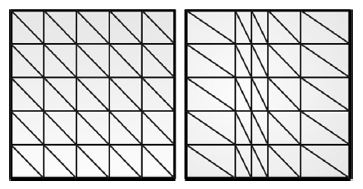
\includegraphics[scale=0.8]{U111_Eta_111.JPG}  \qquad \qquad
		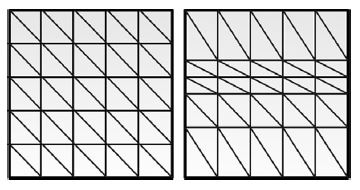
\includegraphics[scale=0.8]{U222_Eta_222.JPG}
	\end{center}
   	\caption{Physical Interpretation of Strain Gradient $\eta_{111}$ and $\eta_{222}$ \cite{lesivcar2017two}}
\end{figure}
\begin{figure}[H]
	\begin{center}
		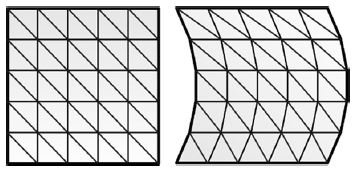
\includegraphics[scale=0.8]{U122_Eta_122.JPG}  \qquad \qquad
		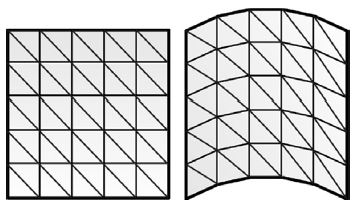
\includegraphics[scale=0.8]{U211_Eta_211.JPG}
   	\caption{Physical Interpretation of Strain Gradient $\eta_{221}$ and $\eta_{112}$ \cite{lesivcar2017two}}		
	\end{center}  
\end{figure}
\begin{figure}[H]
	\begin{center}
		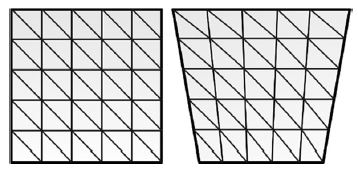
\includegraphics[scale=0.8]{U121_Eta_121.JPG}  \qquad \qquad
		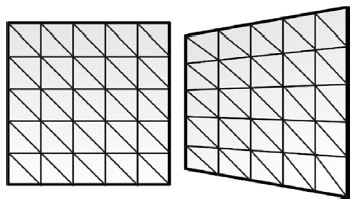
\includegraphics[scale=0.8]{U212_Eta_212.JPG}
   	\caption{Physical Interpretation of Strain Gradient $\eta_{211}$ and $\eta_{122}$ \cite{lesivcar2017two}}
	\end{center}  
\end{figure}

\subsection{E. Amanatidou - Mixed type FEM formulation}
In Mindlin's 1960s theory (2.1), when the problem is formulated in terms of displacements, the governing partial differential Eq.(\ref{first}) is of fourth order. If traditional finite elements are used for the numerical solutions of such problems, then $C^1$ displacements continuity is required at inter elements.
\newline
\newline
Furthermore, E. Amanatidou \cite{amanatidou2002mixed} and et al. developed the alternative Mixed type finite element formulation, in which both displacements and the displacement gradients are used as independent unknowns and their relationship is enforced in an integral sense. In addition to that, this variational formulation can be used for both linear and non-linear strain gradient elasticity theories. In conclusion, this finite elements requires only $C^0$ continuity and simple to formulate and implement into FE program using UEL.   
\newline
\newline
The three equivalent forms strain energy density W given by Mindlin is expressed as,
\begin{equation}
W = \tilde{\mathbf{W}}(\varepsilon,\tilde{\mathbf{\kappa}}) = \hat{\mathbf{W}}(\varepsilon,\hat{\mathbf{\kappa}}) = \bar{\mathbf{W}}(\varepsilon,\bar{\kappa},\bar{\bar \kappa})
\end{equation}
\newline
where the expression $W = \tilde{\mathbf{W}}(\varepsilon,\tilde{\mathbf{\kappa}})$ known as "Type I", the expression $W =\hat{\mathbf{W}}(\varepsilon,\hat{\mathbf{\kappa}}) $ known as "Type II" and the expression $W = \bar{\mathbf{W}}(\varepsilon,\bar{\kappa},\bar{\bar \kappa}) $ known as "Type III".
\newline
\newline
where the Strain energy density for all three forms are represented as,
\newline
\newline
\begin{equation}\label{eleven}
\tilde{\mathbf{W}}(\varepsilon,\tilde{\mathbf{\kappa}}) = \dfrac{1}{2}\lambda\varepsilon_{ii}\varepsilon_{kk} + \mu\varepsilon_{ij}\varepsilon_{ij}+\frac{1}{2}l^2[\lambda\tilde{\kappa_{ijj}}\tilde{\kappa_{ikk}} + \mu(\tilde{\kappa_{ijk}}\tilde{\kappa_{ijk}}+\tilde{\kappa_{ijk}}\tilde{\kappa_{kji}})]
\end{equation}
\begin{equation}
 \hat{\mathbf{W}}(\varepsilon,\hat{\mathbf{\kappa}}) = \dfrac{1}{2}\lambda\varepsilon_{ii}\varepsilon_{kk} + \mu\varepsilon_{ij}\varepsilon_{ij}+\frac{1}{2}l^2(\lambda\tilde{\kappa_{ijj}}\tilde{\kappa_{ikk}}+2\mu\lambda\tilde{\kappa_{ijk}}\tilde{\kappa_{ijk}})
\end{equation}
\begin{equation}
\begin{aligned}
\bar{\mathbf{W}}(\varepsilon,\bar{\kappa},\bar{\bar \kappa}) &= \dfrac{1}{2}\lambda\varepsilon_{ii}\varepsilon_{kk} + \mu\varepsilon_{ij}\varepsilon_{ij} +l^2 [\frac{2}{9}(\lambda+3\mu)\bar{\kappa_{ij}}\bar{\kappa_{ij}}-\frac{2}{9} \lambda \bar{\kappa_{ij}} \bar{\kappa_{ji}} \\
& + \dfrac{1}{2}\lambda \bar{\bar{\kappa_{iij}}} \bar{\bar {\kappa_{kkj}}} + \mu \bar{\bar{ \kappa_{ijk}}} \bar{\bar{ \kappa_{ijk}}} \frac{2}{3}\lambda e_{ijk}\bar{\kappa_{ij}}\bar{\bar {\kappa_{kpp}}}]
\end{aligned}
\end{equation}
\newline
\newline
Amanatidou and Aravas only considered the first form of strain energy density Eq.(\ref{eleven}), which only depends upon conventional strain $ \varepsilon_{ij} $ and higher-order strain-gradient $ \kappa_{ijk} $. 
\newline
\subsubsection{ Stress  }
From the Eq.(\ref{eleven}) we can easily derived the Cauchy stress $\sigma_{ij}$ as,
\begin{equation}\label{fifteen}
\begin{aligned}
\bar{\sigma}_{ij} = \frac{\partial \tilde{\mathbf{W}} }{\partial \varepsilon_{ij}} &=  \lambda\varepsilon_{kk}\delta_{ij} +2\mu\varepsilon_{ij} 
\\
\\
&= \lambda\varepsilon_{kl}\delta_{kl}\delta_{ij} + 2\mu\varepsilon_{kl}\delta_{ik}\delta_{jl} 
\\
\\
&= (\lambda\delta_{kl}\delta_{ij} + 2\mu\delta_{ik}\delta_{jl})\varepsilon_{kl}
\end{aligned}
\end{equation} 
\newline
\newline
Now, it can be easily defined the Second-order tensor $C_{ijkl}$ using the stress-strain relation as,
\begin{equation}\label{sixteen}
{\sigma}_{ij} = C_{ijkl} \varepsilon_{kl} 
\end{equation}
By comparing the Eq.(\ref{fifteen}) and Eq.(\ref{sixteen}),
\begin{equation}\label{onesix}
C_{ijkl} = \lambda\delta_{kl}\delta_{ij} + 2\mu\delta_{ik}\delta_{jl}
\end{equation}
It can be also written in symmetric $3\times3$ Matrix as,
\begin{equation}\label{seventeen}
C = 
\begin{bmatrix}
\lambda+2\mu & \lambda & 0 \\
\lambda & \lambda+2\mu & 0 \\
0 & 0 & \frac{1}{2}\mu
\end{bmatrix}
\end{equation}
\newline
\subsubsection { Higher Order Stress  }
From the Eq.(\ref{eleven}) we can easily derived the Higher Order stress $\mu_{ijk}$ as,
\begin{equation}\label{eighteen}
\begin{aligned}
\tilde{\mu}_{ijk} =  \frac{\partial \tilde{\mathbf{W}} }{\partial \kappa_{ijk}} &= \frac{1}{2}l^2[\lambda \kappa_{ijj}\delta_{ip} \delta_{kq} \delta_{kr} + \lambda \kappa_{ikk}\delta_{ip} \delta_{jq} \delta_{jr} \\
& + 2\mu \kappa_{ijk}\delta_{ip} \delta_{jq} \delta_{kr}  + \mu \kappa_{kji}\delta_{ip} \delta_{jq} \delta_{kr} + \mu \kappa_{ijk}\delta_{kp} \delta_{jq} \delta_{ir} ] \\
\\
&= \frac{1}{2}l^2 [ \lambda \kappa_{pjj}\delta_{qr} + \lambda \kappa_{pkk}\delta_{qr}  +2\mu \kappa_{pqr} + \mu\kappa_{rqq} + \mu\kappa_{rqp}   ] \\ 
\\
&= \frac{1}{2}l^2 [ \lambda\delta_{qr} (\kappa_{pjj}+\kappa_{pkk})   + 2\mu (\kappa_{pqr} + \kappa_{rqp}) ] \\
\\
&= \frac{1}{2}l^2 [ 2\lambda \delta_{qr} \delta_{ip} \delta_{kj} + 2\mu(\delta_{ip} \delta_{jq} \delta_{kr} + \delta_{ir} \delta_{jq} \delta_{kp})  ] \kappa_{ijk}
\\
\\
&= l^2 [ \lambda \delta_{qr} \delta_{ip} \delta_{kj} + \mu(\delta_{ip} \delta_{jq} \delta_{kr} + \delta_{ir} \delta_{jq} \delta_{kp}) ] \kappa_{ijk}
\end{aligned}
\end{equation}
\\
\\
Now, it can be easily derived the Third-order tensor $D_{pqrijk}$ using the Higher order stress and Strain gradient relation as,
\begin{equation}\label{nineteen}
\mu_{pqr} = D_{pqrijk} \kappa_{ijk}
\end{equation}
\\
\\
By, comparing the Eq.(\ref{eighteen}) and Eq.(\ref{nineteen}),
\begin{equation}\label{twenty}
D_{pqrijk} = l^2 [ \lambda \delta_{qr} \delta_{ip} \delta_{kj} + \mu(\delta_{ip} \delta_{jq} \delta_{kr} + \delta_{ir} \delta_{jq} \delta_{kp}) ]
\end{equation}
\\
\\
Now, Eq.(\ref{twenty}) can also be written in matrix notation as following, where $D_{pqrijk}$ is a symmetric $6\times6$ matrix.
\\
\\
\begin{equation}\label{twoone}
D = l^2
\begin{bmatrix}
\lambda + 2\mu & 0 & 0 & 0 & 0 & \frac{\lambda}{2} \\
0 & \mu & 0  & 0  & 0  & \frac{\mu}{2} \\
0 & 0 & \mu & 0  & \frac{\mu}{2}  & 0 \\
0 & 0 & 0 & \lambda + 2\mu & \frac{\lambda}{2} & 0 \\
0 & 0 & \frac{\mu}{2}  & \frac{\lambda}{2} & \frac{\lambda + 3\mu}{4} & 0 \\
 \frac{\lambda}{2} & \frac{\mu}{2} & 0 & 0 & 0 & \frac{\lambda + 3\mu}{4} 
\end{bmatrix}
\end{equation}
\\
\\
So, Eq.(\ref{seventeen}) and Eq.(\ref{twoone}) are the Voigt-notation of the constitutive equation of a general strain gradient solid introduced by Amanatidou and Aravas. 
\newpage
\subsubsection{ Mixed Tpye Elements}
    \begin{figure}[H]
    	\begin{center}
		     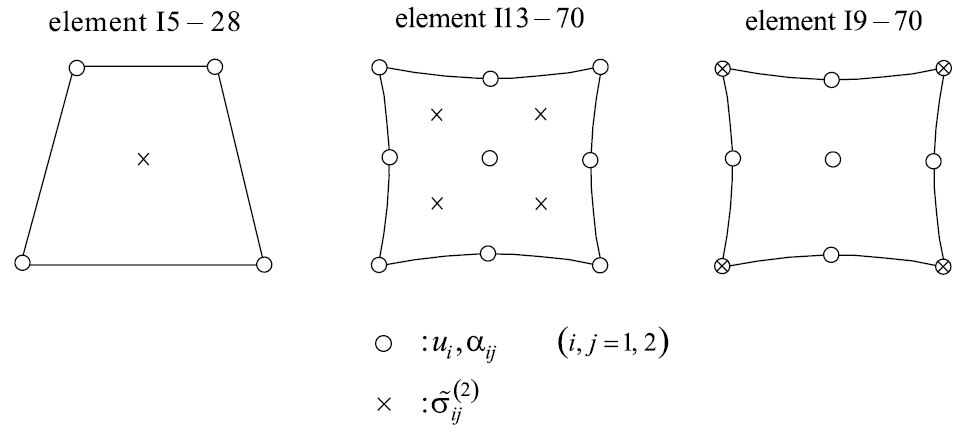
\includegraphics[scale=.65]{Element_mixed_type_formulation_E_Amanatidou.JPG}  	
	    \end{center}  
        \caption{C0-continuous Finite elements for Type I formulation. \cite{amanatidou2002mixed}}   
    \end{figure}
Amanatidou and Aravas presented several elements that can be used in Type-I formulation are shown in above Fig. The elements are shown in Fig. , the corresponding nodal degrees of freedom are u,$\alpha$ and $\sigma$. Finally, Amanatidou and Aravas conclude that, Out of these given elements only the element I9-70 passes the all patch test, whereas the elements I5-28 and I13-70 failed into the patch test.
\\
\subsection{John Y. Shu - Mixed type FEM formulation}
\vspace{0.4cm}
Conventional continuum mechanics theories assume that stress at a material point is a function
of state variables, such as strain, at the same point. This assumption has valid until when the wavelength of a deformation field is much larger than the dominant micro-structural length scale of the material. However, when the two length scales are comparable, this assumption is proved wrong because the material behaviour at any material point is affected by the surrounding material points deformation. Therefore, Fleck—Hutchinson strain gradient plasticity, which falls within the Toupin—Mindlin framework, represent the virtual work in terms of strain gradients and higher order stresses.
\newline
\newline
John Y. Shu \cite{shu1999finite} developed Mixed type FEM formulation of Fleck—Hutchinson strain gradient elasticity theory. They devised $C^0$ continuous elements of mixed type, in which additional nodal degrees of freedom "Relaxed Strain" is introduced and enforce the kinematic constraints between displacement and relaxed strain by Lagrange multipliers.
\newline
\subsubsection{ Modified Virtual Work}
Firstly, for mixed type FEM formulation, they first derive a weak form of the principle of virtual
work suitable for finite element implementation using $C^0$-shape functions. In this modified virtual work only first-order gradients of kinematic quantities involving. In this introduced a second-order tensor $\psi$ and a related third-order tensor $\eta$ such that $\eta_{ijk}$ is defined as,
\\
\begin{equation}\label{twotwo} 
\eta_{ijk} = (\psi_{jk,i}+\psi_{ik,j})/2
\end{equation}
Now, modified weak form virtual work is represented as,
\begin{equation}\label{twothree}
\begin{aligned}
\int\limits_\Omega\! [ \sigma_{ij}\delta\varepsilon_{ij} + \tau_{ijk}\delta\eta_{ijk} + \tau_{ijk,i}(\delta\psi_{jk}-\delta u_{k,j})  ] d\Omega &= \int\limits_\Omega\! [b_k\delta u_k] d\Omega + \int\limits_\Gamma\! [ t_k\delta u_k + n_jr_k\delta\psi_{jk} ] d\Gamma \\
&+ \int\limits_\Gamma\! ( n_i\tau_{ijk} -n_jr_k ) ( \delta\psi_{jk}-\delta u_{k,j} ) d\Gamma
\end{aligned}
\end{equation}
\newline
for arbitrary variations of du and d$\psi$. If $ \psi $ is subjected strictly to the constraint of
$ \delta\psi = \delta u_{k,j} $ into the whole domain $ \Omega $, then as previously discussed, the strict enforcement of this constraint will demand $C^1$ continuous elements. Therefore, to facilitate the use of convenient $C^0$-continuous elements, this constraint is enforced in the following weighted residual manner as,
\begin{equation}\label{twofour}
\int\limits_\Omega\! (\psi_{jk} - u_{k,j})\delta\tau_{ijk,i} d\Omega = 0  \quad (no \quad sum\quad over \quad j \quad and \quad k)
\end{equation}
for an arbitrary variation of the Lagrange multipliers $ \tau_{ijk,i} $. Finally, by denoting the Lagrange multipliers $ \delta \tau_{ijk,i}$ in above equation as $ \delta\rho_{jk} $ the modified virtual work statement Eq.(\ref{twothree}) becomes,
\begin{equation}\label{twofive}
\int\limits_\Omega\! [ \sigma_{ij}\delta\varepsilon_{ij} + \tau_{ijk}\delta\eta_{ijk} + \rho_{jk}(\delta\psi_{jk}-\delta u_{k,j})] d\Omega = \int\limits_\Omega\! [b_k\delta u_k] d\Omega + \int\limits_\Gamma\! [ t_k\delta u_k + n_jr_k\delta\psi_{jk} ] d\Gamma
\end{equation}
and the modified constraint from Eq.(\ref{twofour}) becomes,
\begin{equation}\label{twosix}
\int\limits_\Omega\! (\psi_{jk} - u_{k,j})\delta\rho_{jk}  d\Omega = 0  \quad (no \quad sum\quad over \quad j \quad and \quad k)
\end{equation} 
By considering the above criteria we get the strain energy density in terms of the relaxed strain gradient from Eq.(\ref{two}) as,
\begin{equation}\label{twoseven}
W = \frac{1}{2}\lambda\varepsilon_{ii}\varepsilon_{jj}+\mu\varepsilon_{ij}\varepsilon_{ij} +\frac{1}{2}\mu l^2 ( \eta_{ijk}\eta_{ijk} - \eta_{ijk}\eta_{kji} )
\end{equation}
\\
\subsubsection{ Stress}
From the Eq.(\ref{twoseven}) we can easily derived the Cauchy stress $\sigma_{ij}$ as,
\begin{equation}\label{twoeight}
\begin{aligned}
\bar{\sigma}_{ij} = \frac{\partial \tilde{\mathbf{W}} }{\partial \varepsilon_{ij}} &=  \lambda\varepsilon_{kk}\delta_{ij} +2\mu\varepsilon_{ij} = (\lambda\delta_{kl}\delta_{ij} + 2\mu\delta_{ik}\delta_{jl})\varepsilon_{kl} = C_{ijkl} \varepsilon_{kl}
\end{aligned}
\end{equation} 
So, it yields the same result as given by Eq.(\ref{fifteen}) and Eq.(\ref{sixteen}). Therefore, we can also write the matrix notation of $ C_{ijkl} $ and it also same as Eq.(\ref{seventeen}).
\subsubsection{ Higher-order Stress}
From the Eq.(\ref{twoseven}) we can easily derived the Higher-order stress $\tau_{ijk}$ as,
\begin{equation}\label{twonine}
\begin{aligned}
\tau_{pqr} & = \frac{\partial \tilde{\mathbf{W}} }{\partial \eta_{pqr}} \\
& = \frac{1}{2}\mu l^2 [ 2(\eta_{ijk} \delta_{ip} \delta_{jq} \delta_{kr}) - \eta_{kji} \delta_{ip} \delta_{jq} \delta_{kr} - \eta_{ijk} \delta_{kp} \delta_{jq} \delta_{ir} ] \\
& =  \frac{1}{2}\mu l^2 [ 2(\eta_{pqr}) - \eta_{rqp} -\eta_{rqp} ] \\
& = \mu l^2 [ \eta_{pqr} - \eta_{rqp} ] \\
& = \mu l^2 [ \delta_{lp} \delta_{mq} \delta_{nr} - \delta_{lr} \delta_{mq} \delta_{np} ]  \eta_{lmn}
\end{aligned}
\end{equation}
Now, it can be easily derived the Third-order tensor $D_{pqrlmn}$ using the Higher order stress $ \tau_{pqr} $ and Strain gradient $ \eta_{lmn} $ relation as,
\begin{equation}\label{thirty}
\tau_{pqr} = D_{pqrlmn} \cdot \eta_{lmn}
\end{equation}
By, comparing the Eq.(\ref{twonine}) and Eq.(\ref{thirty}),
\begin{equation}\label{threeone}
D_{pqrlmn} = \mu l^2 [ \delta_{lp} \delta_{mq} \delta_{nr} - \delta_{lr} \delta_{mq} \delta_{np} ]
\end{equation}
Now, Eq.(\ref{twonine}) can also be written in matrix notation as following, where $D_{pqrlmn}$ is a symmetric $6\times6$ matrix.
\begin{equation}\label{threetwo}
D = \mu l^2
\begin{bmatrix}
0 & 0 & 0 & 0 & 0 & 0  \\
0 & 1 & 0  & 0  & 0  & -\frac{1}{2} \\
0 & 0 & 1 & 0  & -\frac{1}{2}  & 0 \\
0 & 0 & 0 & 0 & 0 & 0 \\
0 & 0 & -\frac{1}{2}  & 0 & \frac{1}{4} & 0 \\
0 & -\frac{1}{2} & 0 & 0 & 0 & \frac{1}{4} 
\end{bmatrix}
\end{equation}
So, Eq.(\ref{seventeen}) and Eq.(\ref{threetwo}) are the Voigt-notation of the constitutive equation of a Couple strain gradient solid represented by JOHN Y. SHU, WAYNE E. KING and NORMAN A. FLECK. 
\subsubsection{ Isoparametric elements for the strain gradient solid}
\begin{figure}[H]
	\begin{center}
		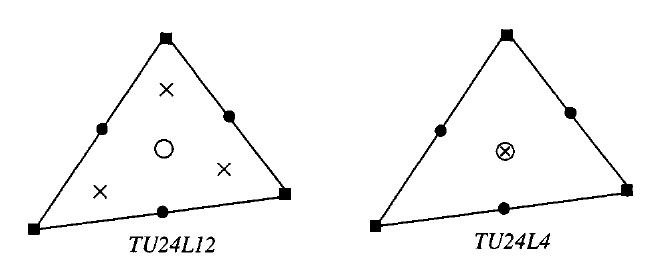
\includegraphics[scale=0.6]{Shu_1_2.JPG}  \qquad
		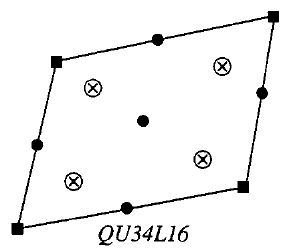
\includegraphics[scale=0.6]{Shu_3.JPG}
	\end{center}  
\end{figure}
\begin{figure}[H]
	\begin{center}
		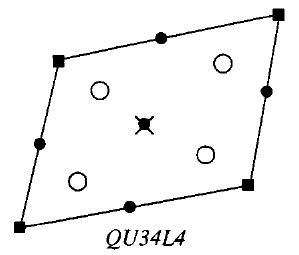
\includegraphics[scale=0.6]{Shu_4.JPG}  \qquad
		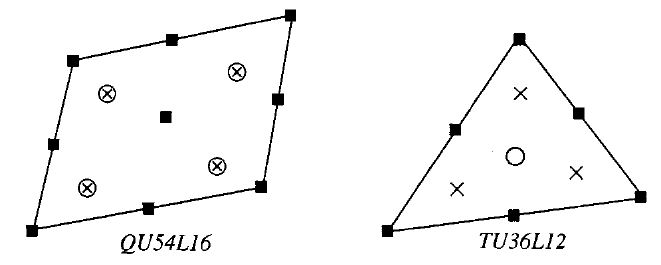
\includegraphics[scale=0.6]{Shu_5_6.JPG}
	\end{center}  
\end{figure}
\begin{figure}[H]
	\begin{center}
		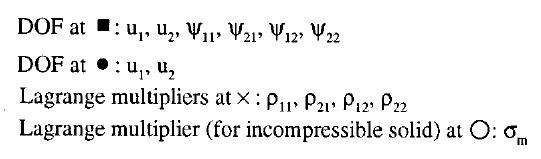
\includegraphics[scale=0.8]{Shu_info.JPG}
	\end{center}  
    \caption{C0-continuous 6 Finite elements for Mixed type of formulation. \cite{shu1999finite}}
\end{figure}
A total of six types of triangular element and quadrilateral element have been developed by JOHN Y. SHU for strain gradient theory. In which Displacement gradients are introduced as extra nodal degrees of freedom in terms of relaxed strain. The kinematic constraints between the relaxed strain and true gradients of displacement are enforced via Lagrange multipliers. All six types of element passed a patch test. However, he recommended QU34L4 elements for practical applications, since it gives precise accuracy than other elements.

\subsubsection{ Finite Element Approaximation  }
From equations Eq.(\ref{twofive}) and Eq.(\ref{twosix}) we can write this equations in matrix notation and also in absence of body forces b.
\begin{equation}\label{thre_23}
\begin{aligned}
0 = &\sum_{e} \delta \bar{u}^{{(e)}^T} \Bigg[\int\limits_{\Omega^{e}}\! (B^{[u]}\sigma^{(e)} - MN^{[\rho^{T}]} \bar{\rho}^{(e)} ) d\Omega - \int\limits_{\Gamma^{(e)}_t}\!  N^{[u]}\bar{t}^{[e]}d\Gamma \Bigg] \\ + &\sum_{e} \delta \bar{\psi}^{{(e)}^T} \Bigg[\int\limits_{\Omega^{e}}\! (B^{[\psi]}\tau^{(e)} - N^{[\psi^{T}]}N^{[\rho^{T}]} \bar{\rho}^{(e)} ) d\Omega - \int\limits_{\Gamma^{(e)}}\!  N^{[\psi]}\bar{r}^{[e]}d\Gamma \Bigg]
\end{aligned}
\end{equation}
It is also same for the constraint by also excluding the body forces.
\begin{equation}\label{thre_234}
\begin{aligned}
\sum_{e} \delta \bar{u}^{{(e)}^T} \int\limits_{\Omega^{e}}\! N^{[\rho]}(N^{[\psi]^{T}}\bar{\psi}^{[e]} - M^T\bar{u}^{(e)} ) d\Omega = 0
\end{aligned}
\end{equation}
So, from equations Eq.(\ref{thre_23}) and Eq.(\ref{thre_234}), we can write the nonlinear internal force vectors are 
\begin{equation}\label{thre_2345}
\begin{aligned}
F(\bar{u}^{(e)},\bar{\rho}^{(e)}) &= \int\limits_{\Omega^{e}}\! (B^{[u]}\sigma^{(e)} - MN^{[\rho^{T}]} \bar{\rho}^{(e)} ) d\Omega \\
R(\bar{\psi}^{(e)},\bar{\rho}^{(e)}) &= \int\limits_{\Omega^{e}}\! (B^{[\psi]}\tau^{(e)} - N^{[\psi^{T}]}N^{[\rho^{T}]} \bar{\rho}^{(e)} ) d\Omega \\
S(\bar{u}^{(e)},\bar{\psi}^{(e)}) &= \int\limits_{\Omega^{e}}\! N^{[\rho]}(N^{[\psi]^{T}}\bar{\psi}^{[e]} - M^T\bar{u}^{(e)} ) d\Omega
\end{aligned}
\end{equation}
we can also write the applied loads in form of vector as below,
\begin{equation}\label{thre_23456}
\begin{aligned}
\psi &= \int\limits_{\Gamma^{(e)}_t}\!  N^{[u]}\bar{t}^{[e]}d\Gamma, \\
\Theta &= \int\limits_{\Gamma^{(e)}}\!  N^{[\psi]}\bar{r}^{[e]}d\Gamma
\end{aligned}
\end{equation}
So, initial system of equation which was solved by Newtion raphson method is,
\begin{equation}\label{thre_234567}
\begin{aligned}
0 &= G(\bar{u}^{(e)},\bar{\rho}^{(e)}) = F(\bar{u}^{(e)},\bar{\rho}^{(e)}) - \psi, \\
0 &= H(\bar{\psi}^{(e)},\bar{\rho}^{(e)}) = R(\bar{\psi}^{(e)},\bar{\rho}^{(e)}) - \Theta, \\
0 &= I(\bar{u}^{(e)},\bar{\psi}^{(e)}) = S(\bar{u}^{(e)},\bar{\psi}^{(e)}) 
\end{aligned}
\end{equation}
Now, from equations (\ref{thre_2345},\ref{thre_23456} and \ref{thre_234567}), we can write the stiffness matrix,solved by the newton raphson scheme,as follow \cite{zybell2012three},
\begin{equation}\label{thre_2345678}
\begin{aligned}
K^{[uu]}  &= \frac{dG}{d\bar{u}^{(e)}} = \int\limits_{\Omega^{e}}\! B^{[u]}\Upsilon B^{[u]^{T}} d\Omega, \\
K^{[\psi\psi]}  &= \frac{dH}{d\bar{\psi}^{(e)}} =\int\limits_{\Omega^{e}}\! B^{[\psi]} \varLambda B^{[\psi]^{T}} d\Omega, \\
K^{[u\rho]}  &= \frac{dG}{d\bar{\rho}^{(e)}}  =\int\limits_{\Omega^{e}}\! M N^{[\rho]^{T}} d\Omega, \\
K^{[\psi\rho]}  &= \frac{dH}{d\bar{\rho}^{(e)}} =\int\limits_{\Omega^{e}}\! N^{[\psi]} N^{[\rho]^{T}} d\Omega
\end{aligned}
\end{equation}
\newpage
\section{FEM Implementation}
In subsection "John Y. Shu - Mixed type FEM formulation", there are 6 different triangular element and quadrilateral element represented out of which element QU34L4 is recommended for practical applications. so here we will use the QU34L4 element in order to implement strain gradient theory. So, use this specific mixed fem formulation \cite{Lzybell2007} is most challenging task for me.
\\
\subsection{QU34L4 - ELEMENT}
This QU34L4 is Shown in below Fig. ,which contains total 9 nodes and 38 degrees of freedom. In this element there are two displacements DOF $ u_1 $ and $ u_2  $ at each nodes of it. There are newly introduced relaxed strain DOF $ \psi_{11} $,$ \psi_{21} $,$ \psi_{12} $ and $ \psi_{22} $ at each corner nodes of it. In addition to that there are also four Lagrange multipliers $ \rho_{11} $,  $ \rho_{21} $, $ \rho_{12} $ and $ \rho_{22} $,  which are assumed to be constant throughout the element. So, in QU34L4 Q stands for nine-noded isoparametric quadrilateral element, where U stands for number of DOF related to the displacement which are total 34 in this element, where L stands for Lagrange multipliers which are total 4 in this element. 
\begin{figure}[H]
	\begin{center}
		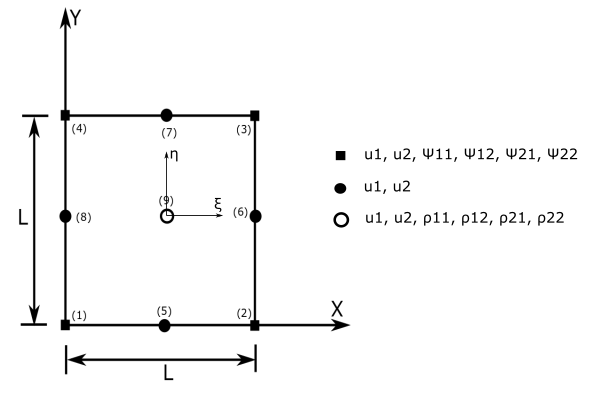
\includegraphics[scale=0.8]{ele_1.png}
	\end{center} 
    \caption{C0-continuous QU34L4 Element.} 
\end{figure}
Displacements $ u_1 $,$ u_2 $ are interpolated using standard quadratic shape functions in terms of the area co-ordinates. Relaxed displacement gradients $ \psi_{11} $,$ \psi_{21} $,$ \psi_{12} $ and $ \psi_{22} $ are interpolated linearly. The different interpolation is motivated by the consideration that the true displacement gradients $ \varepsilon_{ij} $ will depend linearly
on the co-ordinates if all sides of the element are straight.
\subsection{Degrees of Freedom(DOF)}
In this section we derive the finite element shape function and its derivatives for the different DOF - displacements and relaxed strain. In this we also defined matrices for langrange multipliers and also established the matrices containing the shape functions and its derivatives \cite{Lzybell2007}.
\subsubsection{ Displacement DOF}
As discussed in above section, there are two displacements DOF $u_1$ and $u_2$ at each nodes. From the weak of modified virtual work we can derive the relation between global displacements and nodal-displacement as,
\\
\\
\begin{equation}\label{threethree}
u^{(e)}=
\begin{bmatrix}
u_1^{(e)}\\
u_2^{(e)}
\end{bmatrix}
=N^{[u]^{\textbf{T}}}\cdot \hat{u}^{(e)}
\end{equation}
\\
\\
where $\hat{u}_{(e)}$ is defined in terms of vector as,
\begin{equation}\label{threefour}
\hat u^{(e)}=
\begin{bmatrix}
u_1^{(1)}&u_2^{(1)}&u_1^{(2)}&u_2^{(2)}&\cdots &\cdots u_1^{(9)} u_2^{(9)}
\end{bmatrix}
\end{equation}
\\
In QU34L4 element, as discussed earlier $u_i$ are interpolated using standard quadratic shape functions in terms of the area co-ordinates. So here we derived the shape functions for nine-nodded element in coordinates $\xi$ and $\omega$.
\\
\\
\begin{equation}\label{threefive}
\begin{aligned}
N^{[U]^{(1)}} &= \dfrac{1}{4}\xi(\xi-1)\omega(\omega-1)  \\
N^{[U]^{(2)}} &= \dfrac{1}{4}\xi(\xi+1)\omega(\omega-1)  \\
N^{[U]^{(3)}} &= \dfrac{1}{4}\xi(\xi+1)\omega(\omega+1)  \\
N^{[U]^{(4)}} &= \dfrac{1}{4}\xi(\xi-1)\omega(\omega+1)  \\
N^{[U]^{(5)}} &= \dfrac{1}{2}(1-\xi^2)\omega(\omega-1)   \\
N^{[U]^{(6)}} &= \dfrac{1}{2}\xi(\xi+1)(1-\omega^2)  \\
N^{[U]^{(7)}} &= \dfrac{1}{2}(1-\xi^2)\omega(\omega+1)  \\
N^{[U]^{(8)}} &= \dfrac{1}{2}\xi(\xi-1)(1-\omega^2) \\
N^{[U]^{(9)}} &= (1-\xi^2)(1-\omega^2)  \\
\end{aligned}
\end{equation}
\\
\\
From equations Eq.(\ref{threethree}), Eq.(\ref{threefour}) and Eq.(\ref{threefive}) we can assemble the shape matrix as following,
\begin{equation}\label{threesix}
N^{[u]^{T}}=
\begin{bmatrix}
N^{[u]^{(1)}}&0&N^{[u]^{(2)}}&0&\cdots &\cdots& N^{[u]^{(9)}}&0 \\
0&N^{[u]^{(1)}}&0&N^{[u]^{(2)}}&\cdots &\cdots& 0&N^{[u]^{(9)}}
\end{bmatrix}
\end{equation}
\newpage
Now we have shape functions, so in next step we derive the local derivatives of the shape functions with respect to $\xi$ and $\omega$. 
\\
\\
The local derivatives of shape function with respect to area coordinates $\xi$ and $\omega$ is given as, 
\begin{equation}\label{threeseven}
N^{[U]^{(i)}}_{,\xi} = \dfrac{\partial N^{[U]^{(i)}} }{\partial \xi}
\end{equation}
\begin{equation}\label{threeeight}
N^{[U]^{(i)}}_{,\omega} = \dfrac{\partial N^{[U]^{(i)}} }{\partial \omega}
\end{equation}
\\
\\
From Eq.(\ref{threeseven}) we can get the local derivatives w.r.t  $\xi$ as,
\begin{equation}\label{threenine}
\begin{aligned}
N_{,\xi}^{[U]^{(1)}} &= -\dfrac{1}{2}\xi\omega-\dfrac{1}{4}\omega^2+\dfrac{1}{4}\omega+\dfrac{1}{2}\xi\omega^2  \\
N_{,\xi}^{[U]^{(2)}} &= -\dfrac{1}{2}\xi\omega+\dfrac{1}{4}\omega^2-\dfrac{1}{4}\omega+\dfrac{1}{2}\xi\omega^2  \\
N_{,\xi}^{[U]^{(3)}} &= \dfrac{1}{2}\xi\omega+\dfrac{1}{4}\omega^2+\dfrac{1}{4}\omega+\dfrac{1}{2}\xi\omega^2 \\
N_{,\xi}^{[U]^{(4)}} &= \dfrac{1}{2}\xi\omega-\dfrac{1}{4}\omega^2-\dfrac{1}{4}\omega+\dfrac{1}{2}\xi\omega^2 \\
N_{,\xi}^{[U]^{(5)}} &= \xi\omega-\xi\omega^2 \\
N_{,\xi}^{[U]^{(6)}} &= \xi-\xi\omega^2+\dfrac{1}{2}-\dfrac{1}{2}\omega^2 \\
N_{,\xi}^{[U]^{(7)}} &= -\xi\omega-\xi\omega^2 \\
N_{,\xi}^{[U]^{(8)}} &= \xi-\xi\omega^2-\dfrac{1}{2}+\dfrac{1}{2}\omega^2 \\
N_{,\xi}^{[U]^{(9)}} &= -2\xi+2\xi\omega^2 \\
\end{aligned}
\end{equation}
\\
From Eq.(\ref{threeeight}) we can get the local derivatives w.r.t  $\omega$ as,
\begin{equation}\label{fourty}
\begin{aligned}
N_{,\omega}^{[U]^{(1)}} &= -\dfrac{1}{2}\xi\omega-\dfrac{1}{4}\xi^2+\dfrac{1}{4}\xi+\dfrac{1}{2}\xi^2\omega \\
N_{,\omega}^{[U]^{(2)}} & = \dfrac{1}{2}\xi\omega-\dfrac{1}{4}\xi^2-\dfrac{1}{4}\xi+\dfrac{1}{2}\xi^2\omega \\
N_{,\omega}^{[U]^{(3)}} &= \dfrac{1}{2}\xi\omega+\dfrac{1}{4}\xi^2+\dfrac{1}{4}\xi+\dfrac{1}{2}\xi^2\omega \\
N_{,\omega}^{[U]^{(4)}} &= -\dfrac{1}{2}\xi\omega+\dfrac{1}{4}\xi^2-\dfrac{1}{4}\xi+\dfrac{1}{2}\xi^2\omega \\
N_{,\omega}^{[U]^{(5)}} &= \dfrac{1}{2}\xi^2-\dfrac{1}{2}-\xi^2\omega+\omega \\
N_{,\omega}^{[U]^{(6)}} &= -\xi^2\omega-\xi\omega \\
N_{,\omega}^{[U]^{(7)}} &=  -\dfrac{1}{2}\xi^2+\dfrac{1}{2}-\xi^2\omega+\omega \\
N_{,\omega}^{[U]^{(8)}} &= -\xi^2\omega+\xi\omega \\
N_{,\omega}^{[U]^{(9)}} &= -2\omega+2\xi^2\omega \\
\end{aligned}
\end{equation}
\\
Taking the equations above into consideration, the displacement gradient in the element is derived as following,
\begin{equation}\label{fourone}
\nabla u^{(e)}=
\begin{Bmatrix}
	u_{1,1}^{(e)} \\
	\\
	u_{1,2}^{(e)} \\
	\\
	u_{2,1}^{(e)} \\
	\\
	u_{2,2}^{(e)} 
\end{Bmatrix}
=M^{[u]^{\textbf{T}}}u^{(e)}
\end{equation}
\\
So here in Eq.(\ref{fourone}), the $u_{1,2}$ and $u_{2,1}$ are not same as in consideration of normal strain, where we considered $\varepsilon_{1,2}$ and $ \varepsilon_{2,1}$ are same.
\\
\\
From Eq.(\ref{threefour}) and Eq.(\ref{fourone}), we can defined the Displacements Gradient Matrix as following, 
\begin{equation}\label{fourtwo}
M^{[u]^\textbf{T}}=
\begin{bmatrix}
N_{,1}^{[u]^{(1)}}&0&N_{,1}^{[u]^{(2)}}&0&\cdots &\cdots& N_{,1}^{[u]^{(9)}}&0 \\
N_{,2}^{[u]^{(1)}}&0&N_{,2}^{[u]^{(2)}}&0&\cdots &\cdots& N_{,2}^{[u]^{(9)}}&0 \\
0&N_{,1}^{[u]^{(1)}}&0&N_{,1}^{[u]^{(2)}}&\cdots &\cdots& 0&N_{,1}^{[u]^{(9)}} \\
0&N_{,2}^{[u]^{(1)}}&0&N_{,2}^{[u]^{(2)}}&\cdots &\cdots& 0&N_{,2}^{[u]^{(9)}}
\end{bmatrix}
\end{equation}
\\
\\
Now, we can derived the true strain matrix as following,
\begin{equation}\label{fourthree}
\varepsilon^{(e)}=
\begin{Bmatrix}
\varepsilon_{11}^{(e)} \\
\\
\varepsilon_{22}^{(e)}  \\
\\
\gamma_{12}^{(e)}  \\ 
\end{Bmatrix}
\approx B^{[u]^{\textbf{T}}}u^{(e)}
\end{equation}
\\
From Eq.(\ref{threefour}) and Eq.(\ref{fourthree}), we can defined the differential Matrix $B^u$, which contains the global derivatives of shape functions as following, 
\begin{equation}\label{fourfour}
B^{[u]^\textbf{T}}=
\begin{bmatrix}
	N_{,1}^{[u]^{(1)}}&0&N_{,1}^{[u]^{(2)}}&0&\cdots &\cdots& N_{,1}^{[u]^{(9)}}&0 \\
	0&N_{,2}^{[u]^{(1)}}&0&N_{,2}^{[u]^{(2)}}&\cdots &\cdots& 0&N_{,2}^{[u]^{(9)}} \\
	N_{,2}^{[u]^{(1)}}&N_{,1}^{[u]^{(1)}}&N_{,2}^{[u]^{(2)}}&N_{,1}^{[u]^{(2)}}&\cdots &\cdots& N_{,2}^{[u]^{(9)}}&N_{,1}^{[u]^{(9)}}
\end{bmatrix}
\end{equation}
\\
\\
In both the Eq.(\ref{fourtwo}) and Eq.(\ref{fourfour}), it can be seen that there $N_{,1}$ and $N_{,2}$ which are represented as $N_{,1}^{[u]^{(i)}} = \dfrac{\partial N^{[u]^{(i)}}}{\partial x_1}$ and $N_{,2}^{[u]^{(i)}} = \dfrac{\partial N^{[u]^{(i)}}}{\partial x_2}$, which are global derivatives of shape functions related to displacements DOF. which can not be calculated directly since the shape functions are set up in the local coordinate system.
\subsubsection{ Relaxed Strain DOF}
As discussed in above section, there are four relaxed strain DOF $\psi_{11}$,$\psi_{21}$,$\psi_{12}$ and $\psi_{22}$,  at each corned nodes. Now, we can derive the relation between global relaxed strain and nodal-relaxed strain as,
\\
\begin{equation}\label{fourfive}
\psi^{(e)}=
\begin{Bmatrix}
\psi_{11}^{(e)} \\
\\
\psi_{21}^{(e)} \\
\\
\psi_{12}^{(e)} \\
\\
\psi_{22}^{(e)}
\end{Bmatrix}
=N^{[\psi]^{\textbf{T}}} \hat{\psi}^{(e)}
\end{equation}
\\
\\
where, nodal relaxed strain vector $\hat{\psi}^{(e)}$ is defined as following,
\begin{equation}\label{foursix}
\hat{\psi}^{(e)^{\textbf{T}}}=
\begin{bmatrix}
\psi_{(11)}^{(1)}&\psi_{(21)}^{(1)}&\psi_{(12)}^{(1)}&\psi_{(22)}^{(1)}&\cdots &\cdots& \psi_{(11)}^{(4)}&\psi_{(21)}^{(4)}&\psi_{(12)}^{(4)}&\psi_{(22)}^{(4)}
\end{bmatrix}
\end{equation}
\\
Now, defined the shape functions for the relaxed strain. As discussed earlier, in QU34L4 element $\psi_i$ are interpolated using standard bi-linear shape functions in terms of the area coordinates $\xi$ and $\omega$.
\\
\\
\begin{equation}\label{fourseven}
\begin{aligned}
N^{[\psi]^{(1)}} &= \dfrac{1}{4}(1-\xi)(1-\omega) \\
N^{[\psi]^{(2)}} &= \dfrac{1}{4}(1+\xi)(1-\omega) \\ 
N^{[\psi]^{(3)}} &= \dfrac{1}{4}(1+\xi)(1+\omega) \\
N^{[\psi]^{(4)}} &= \dfrac{1}{4}(1-\xi)(1+\omega) \\
\end{aligned}
\end{equation}
\\
\\
Now, considering the equations Eq.(\ref{fourfive}), Eq.(\ref{foursix}) and Eq.(\ref{fourseven}) we can assemble the shape matrix for the relaxed strain degree of freedom as following,
\\
\\
\begin{equation}\label{foureight}
N^{[\psi]^\textbf{T}}=
\begin{bmatrix}
N^{{\psi}^{(1)}}&0&0&0&\cdots&\cdots&N^{{\psi}^{(4)}}&0&0&0 \\
0&N^{{\psi}^{(1)}}&0&0&\cdots&\cdots&0&N^{{\psi}^{(4)}}&0&0 \\
0&0&N^{{\psi}^{(1)}}&0&\cdots&\cdots&0&0&N^{{\psi}^{(4)}}&0 \\
0&0&0&N^{{\psi}^{(1)}}&\cdots&\cdots&0&0&0&N^{{\psi}^{(4)}} 
\end{bmatrix}
\end{equation}
\\
\\
Now we have shape functions for relaxed strain DOF Eq.(\ref{fourseven}), so in next step we derive the local derivatives of the shape functions with respect to $\xi$ and $\omega$. 
\\
The local derivatives of shape function with respect to are coordinates $\xi$ and $\omega$ is given as, 
\begin{equation}\label{fournine}
N^{[\psi]^{(i)}}_{,\xi} = \dfrac{\partial N^{[\psi]^{(i)}} }{\partial \xi}
\end{equation}
\begin{equation}\label{fifty}
N^{[\psi]^{(i)}}_{,\omega} = \dfrac{\partial N^{[\psi]^{(i)}} }{\partial \omega}
\end{equation}
\\
From Eq.(\ref{fournine}) we can get the local derivatives w.r.t  $\xi$ as,
\begin{equation}
\begin{aligned}
N_{,\xi}^{[\psi]^{(1)}} &= \dfrac{1}{4}(-1+\omega) \\
N_{,\xi}^{[\psi]^{(2)}} &= \dfrac{1}{4}(1-\omega) \\
N_{,\xi}^{[\psi]^{(3)}} &= \dfrac{1}{4}(1+\omega) \\
N_{,\xi}^{[\psi]^{(4)}} &= \dfrac{1}{4}(-1-\omega) \\
\end{aligned}
\end{equation}
\\
From Eq.(\ref{fifty}) we can get the local derivatives w.r.t  $\omega$ as,
\begin{equation}
\begin{aligned}
N_{,\omega}^{[\psi]^{(1)}} &= \dfrac{1}{4}(-1+\xi) \\
N_{,\omega}^{[\psi]^{(2)}} &= \dfrac{1}{4}(-1-\xi) \\
N_{,\omega}^{[\psi]^{(3)}} &= \dfrac{1}{4}(1+\xi) \\
N_{,\omega}^{[\psi]^{(4)}} &= \dfrac{1}{4}(1-\xi) \\
\end{aligned}
\end{equation}
\\
Now, we defined the strain gradient using the differential matrix Eq.(\ref{fivefour}) and nodal relaxed strain Eq.(\ref{foursix})  
\begin{equation}\label{fivethree}
\eta^{(e)}=
\begin{Bmatrix}
	\eta_{111}^{(e)} \\
	\\
	\eta_{221}^{(e)} \\
	\\
	\eta_{112}^{(e)} \\
	\\
	\eta_{222}^{(e)} \\
	\\
	\phi_{1}^{(e)} \\
	\\
	\phi_{2}^{(e)}
\end{Bmatrix}
\thickapprox B^{[\psi]^{\textbf{T}}}\psi^{(e)}
\end{equation}
\\
Form, considering Eq.(\ref{foursix}) and Eq.(\ref{fivethree}) now we can defined the differential matrix $B^\psi$ as following,
\begin{equation}\label{fivefour}
B^{[\psi]^\textbf{T}}=
\begin{bmatrix}
N_{,1}^{{[\psi]}^{(1)}}&0&0&0&\cdots&\cdots&N_{,1}^{{[\psi]}^{(4)}}&0&0&0 \\
0&N_{,2}^{{[\psi]}^{(1)}}&0&0&\cdots&\cdots&0&N_{,2}^{{[\psi]}^{(4)}}&0&0 \\
0&0&N_{,1}^{{[\psi]}^{(1)}}&0&\cdots&\cdots&0&0&N_{,1}^{{[\psi]}^{(4)}}&0 \\
0&0&0&N_{,2}^{{[\psi]}^{(1)}}&\cdots&\cdots&0&0&0&N_{,2}^{{[\psi]}^{(4)}} \\
N_{,2}^{{[\psi]}^{(1)}}&N_{,1}^{{[\psi]}^{(1)}}&0&0&\cdots&\cdots&N_{,2}^{{[\psi]}^{(4)}}&N_{,1}^{{[\psi]}^{(4)}}&0&0 \\
0&0&N_{,2}^{{[\psi]}^{(1)}}&N_{,1}^{{[\psi]}^{(1)}}&\cdots&\cdots&0&0&N_{,2}^{{[\psi]}^{(4)}}&N_{,1}^{{[\psi]}^{(4)}} 
\end{bmatrix}
\end{equation}
\\
In this above Eq.(\ref{fivefour}), it can be seen that there $N_{,1}^\psi$ and $N_{,2}^\psi$ which are represented as $N_{,1}^{[\psi]^{(i)}} = \dfrac{\partial N^{[\psi]^{(i)}}}{\partial x_1}$ and $N_{,2}^{[\psi]^{(i)}} = \dfrac{\partial N^{[\psi]^{(i)}}}{\partial x_2}$, which are global derivatives of shape functions related to displacements DOF. which can not be calculated directly since the shape functions are set up in the local coordinate system $ \xi$ and $ \omega$.
\subsubsection{ Langrange Multiplier}
The Lagrange multipliers in the element $ \rho^{(e)}$ are defined as,
\begin{equation}
\rho^{(e)}=
\begin{Bmatrix}
\rho_{11}^{(e)} \\
\\
\rho_{21}^{(e)} \\
\\
\rho_{12}^{(e)} \\
\\
\rho_{22}^{(e)}
\end{Bmatrix}
=N^{[\rho]^{\textbf{T}}}\rho^{(e)}
\end{equation}
\\
As discussed earlier in above section, it is assumed that  Lagrange multipliers constant throughout the element they are only existent at the middle node and therefore, the shape functions matrix for it defined as,
\begin{equation}
N^{[\rho]}=
\begin{bmatrix}
1&0&0&0 \\
\\
0&1&0&0 \\
\\
0&0&1&0 \\
\\
0&0&0&1
\end{bmatrix}
\end{equation}
\newpage
\section{Verification of model without Gradient term}
After completely programmed the Strain Gradient theory for FEM model into Fortran programming language. I tried to run this code with ABAQUS. And Surprisingly, I got the different errors, out of which main errors are Convergence errors, NAN error and singularities error. In conclusion of that I have decided to debug my code from the scratch. Therefore, I have decided to check for the simpler case which is Mechanical Displacement degree of freedom. So first i wanted to check that my code is correctly running for the Displacement degree of freedom.
\\
\\
So, I have just commented all the terms which is related to gradient term i.e. which is related to the relaxed strain and Lagrange degree of freedom. After that I have implement my code to the plate-720 geometry which is explained in detailed in later sections.
\\
\\ 
Now, I have implement the my code which is correctly running after the removing of many hurdles in terms of programming error. Here, I representing the my code results for simpler loading conditions and compare it with the ABAQUS results.  
\\
\\
So, here I represent the displacement results of ABAQUS with simpler loading i.e. $ 1 \% $ of strain in positive Y direction with my results without including the gradient terms and any other degrees of freedom.
\begin{figure}[H]
	\begin{center}
		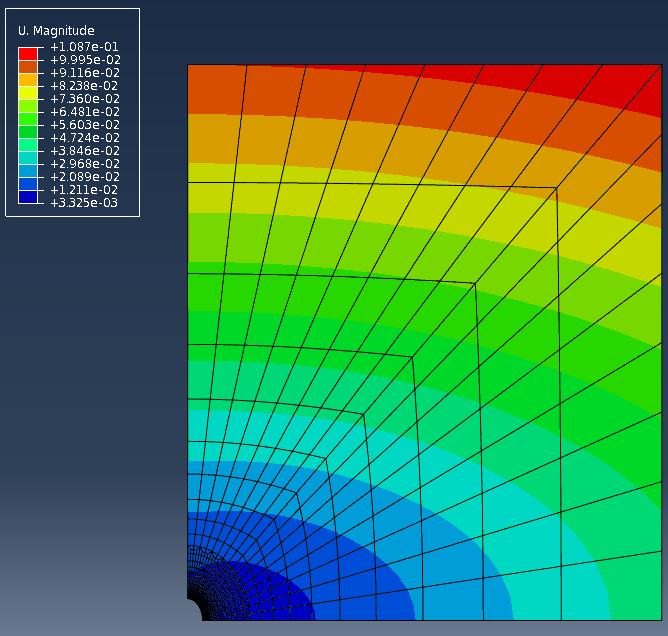
\includegraphics[scale=0.4]{ABAQUS_result.png}  
	\end{center}  
    \caption{Displacement visualization of ABAQUS Model.}
\end{figure}
\begin{figure}[H]
	\begin{center}
		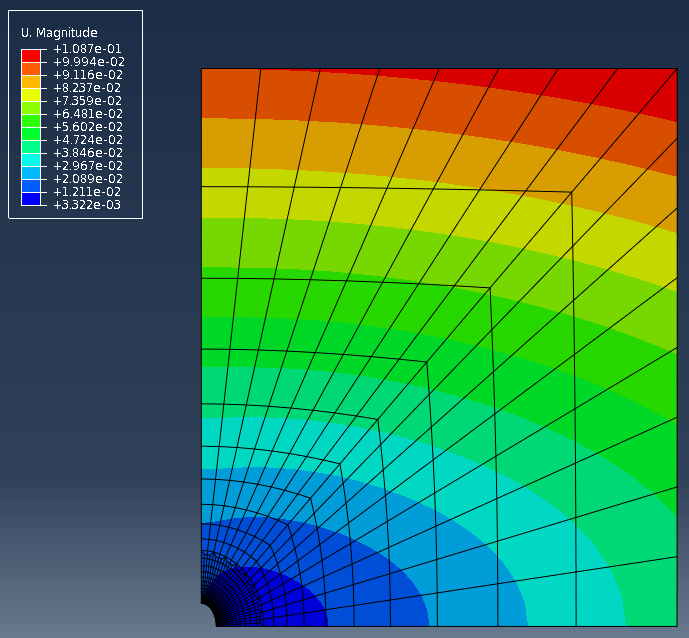
\includegraphics[scale=0.4]{MY_code_result_1.png} 
	\end{center}  
    \caption{Displacement visualization of Strain Gradient Model.}
\end{figure}
So, here I represent the Stress results of ABAQUS with simpler loading i.e. $ 1 \% $ of displacement in positive Y direction with my results without including the gradient terms and any other degrees of freedom. In the second fig I have represent the complex part of geometry.
\begin{figure}[H]
	\begin{center}
		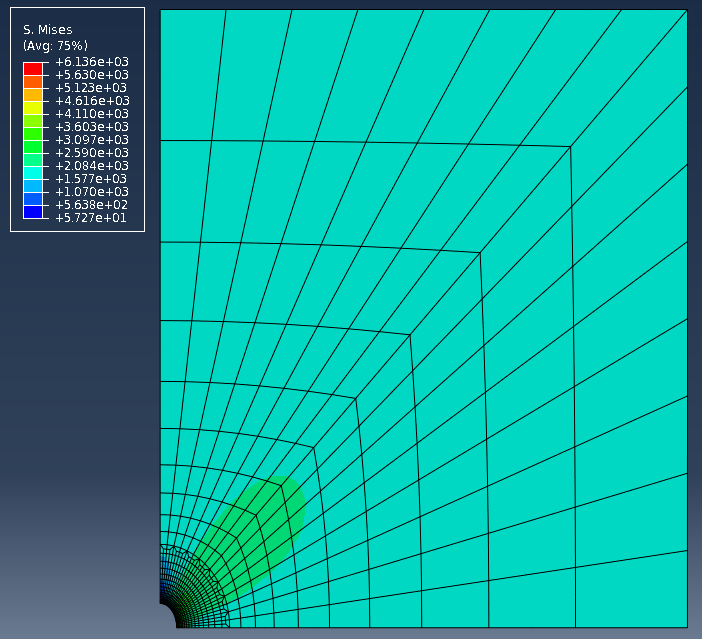
\includegraphics[scale=0.4]{ABAQUS_result_stress.png} 
		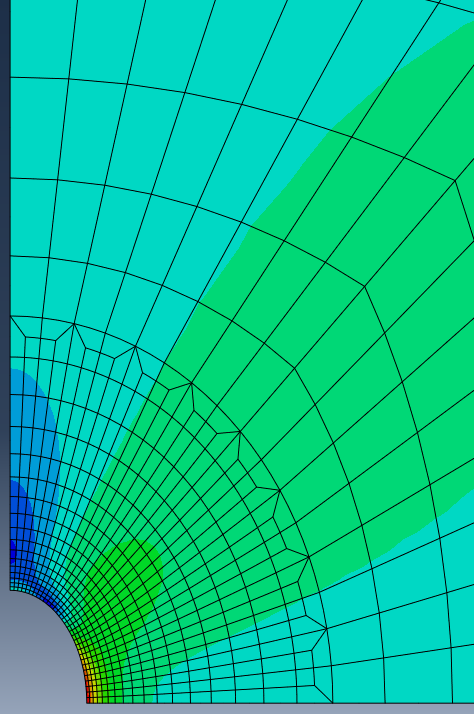
\includegraphics[scale=0.35]{ABAQUS_result_stress_crp.png} 
	\end{center}  
    \caption{Stress visualization of ABAQUS Model.}
\end{figure}
\begin{figure}[H]
	\begin{center}
		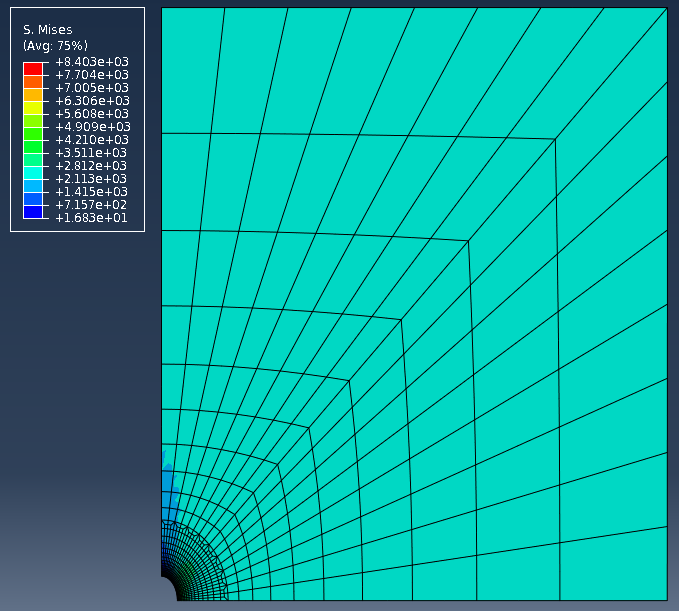
\includegraphics[scale=0.4]{MY_code_result_stress.png} \quad
		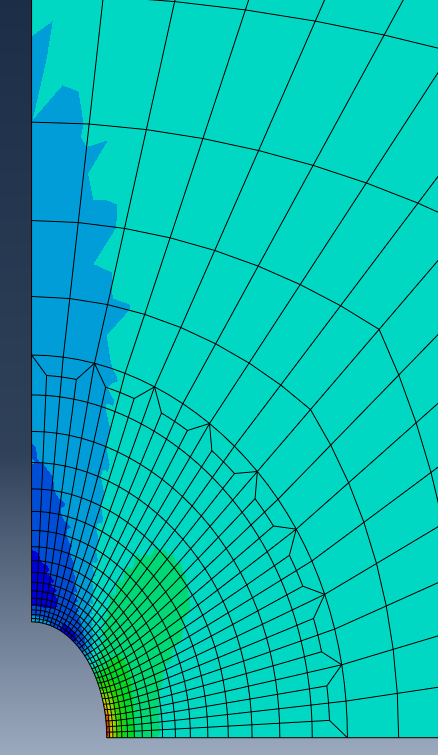
\includegraphics[scale=0.32]{MY_code_result_stress_crp.png}
	\end{center}  
   \caption{Stress visualization of Strain Gradient Model.}
\end{figure}

\newpage
\section{Verification of Model Plate-720}
As of described in E. Amanatidou - Mixed type FEM formulation, they have used the PLATE-720 which contains the 720 elements and 2983 nodes. Using this geometry they try to find the stress concentration factor and plot the stress concentration factor for different microstructural length.
\\
So, here I have used the same geometry i.e. Plate with domain length of 10 and hole radius is 0.333. I also mesh it as same as described in that paper with also transition of fine mesh into the coarse mesh, which is at 1.332 from the centre of the hole.   
\begin{figure}[H]
	\begin{center}
		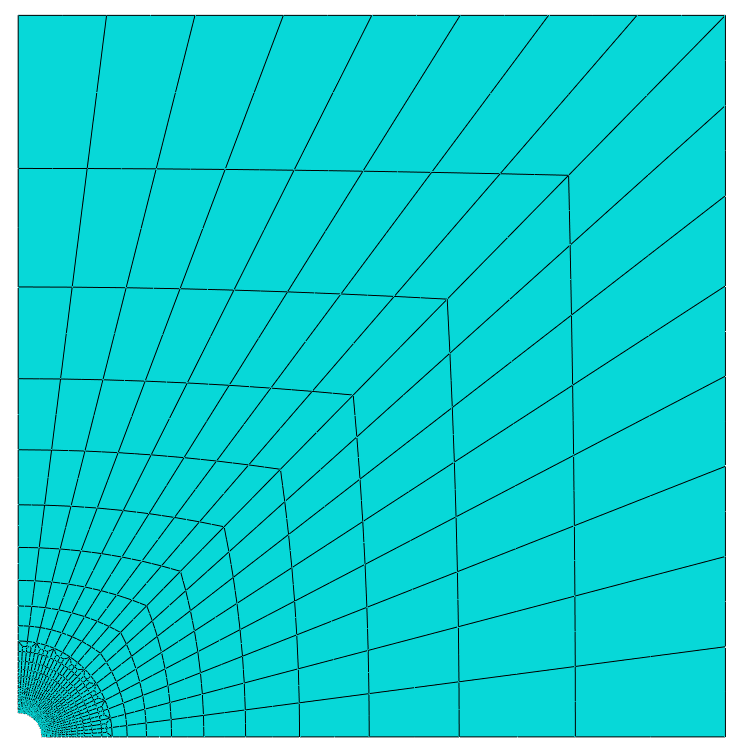
\includegraphics[scale=0.35]{mesh_part.png} 
	\end{center}  
   \caption{Meshed Plate-720 with hole in the left-bottom corner.}
\end{figure}
Here, I specifically represent the fine mesh around the hole and also the transition of mesh from fine mesh to coarse mesh at specific position from the centre of the hole.
\begin{figure}[H]
	\begin{center}
		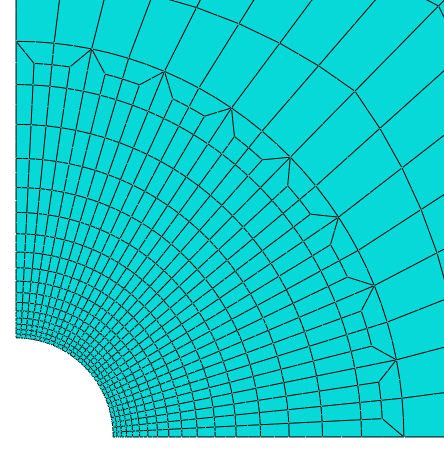
\includegraphics[scale=0.38]{fine_mesh_part.png} 
	\end{center} 
   \caption{Fine mesh and Transition in Plate-720.} 
\end{figure}
Now, the Plate-720 is checked under the tensile loading. Therefore the left edge nodes are fixed in x direction so $U_x = 0$ and bottom edge nodes are fixed in y direction so $U_y = 0$. Now the predefined displacement to the Upper edge nodes are given equal to the 0.1 mm. So now Plate-720 is under tensile loading. In following some strain gradients and higher order stress results are shown as visualize in ABAQUS. From that I conclude that the strain gradient effect is depend on the size of the geometry and also size of the meshes. Here in Plate-720, it is seen that there is hole at the lower-left corner and there is also fine mesh, so there is most probability to getting Strain Gradients and Higher order stresses in element. So the highest strain gradient is seen at X=0.3333 mm and Y=0 mm.
\vspace{3cm} 
\begin{figure}[H]
	\begin{center}
		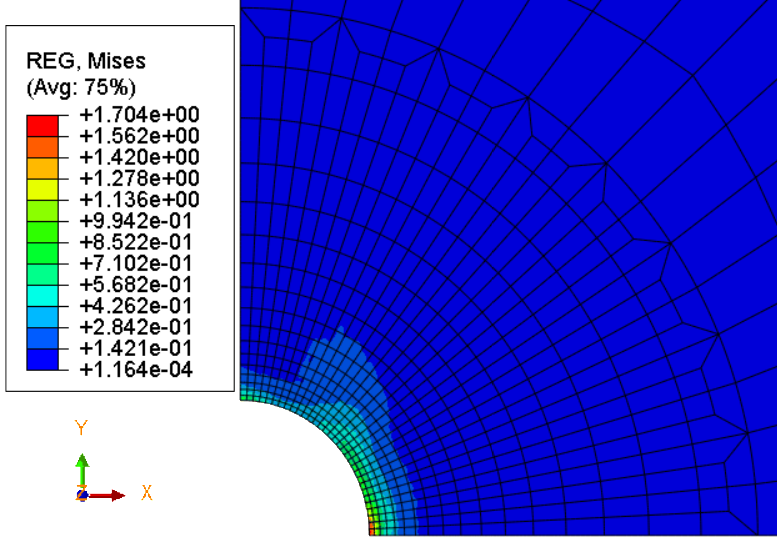
\includegraphics[scale=0.9]{full_grad_crop.png} 
	\end{center}  
   \caption{Strain Gradient Visualization in Plate-720.}
\end{figure}
\begin{figure}[H]
	\begin{center}
		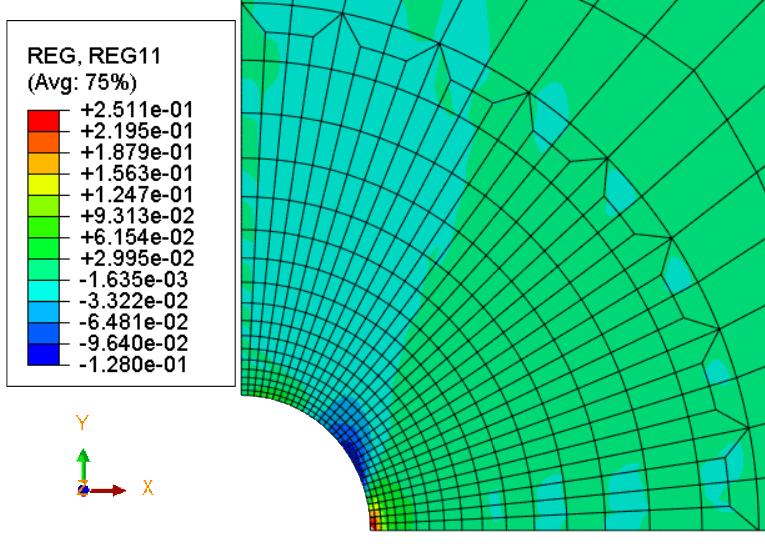
\includegraphics[scale=0.9]{Reg11_crop.png} 
	\end{center}  
   \caption{Visualization of Strain Gradient $\eta_{111} $}
\end{figure}
\begin{figure}[H]
	\begin{center}
		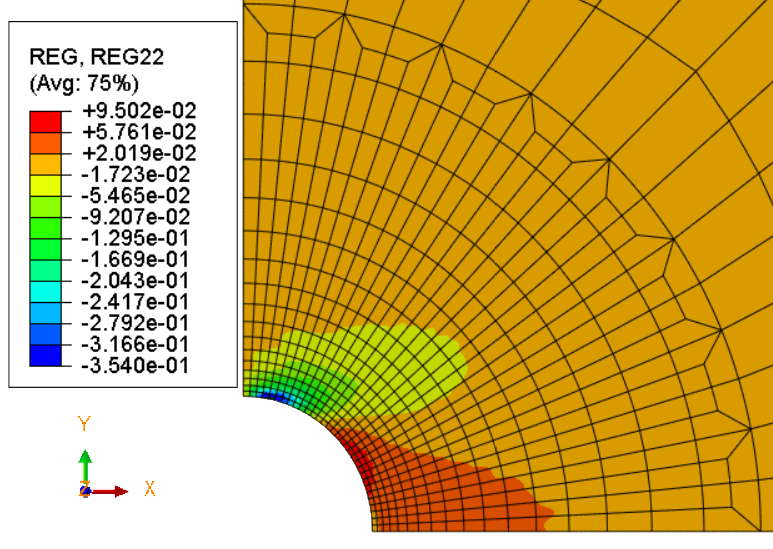
\includegraphics[scale=0.9]{Reg22_crop.png} 
	\end{center}  
   \caption{Visualization of Strain Gradient $\eta_{221} $}
\end{figure}
\begin{figure}[H]
	\begin{center}
		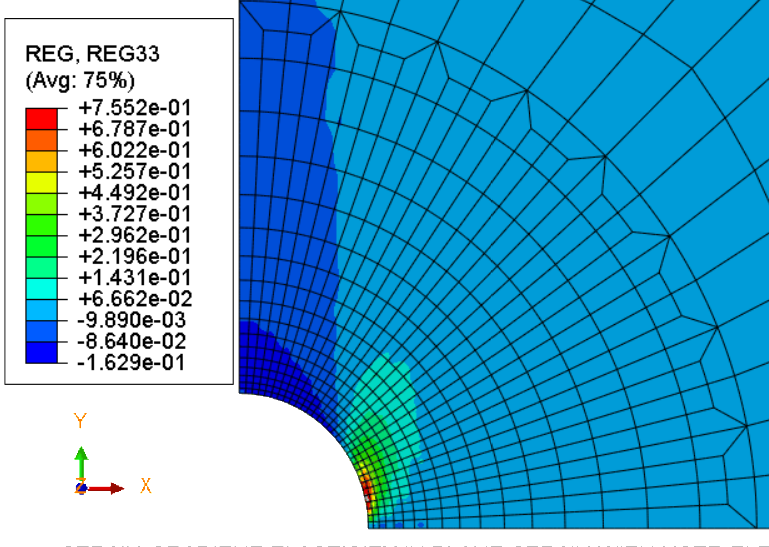
\includegraphics[scale=0.9]{Reg33_crop.png} 
	\end{center}  
   \caption{Visualization of Strain Gradient $\eta_{112} $}
\end{figure}
\begin{figure}[H]
	\begin{center}
		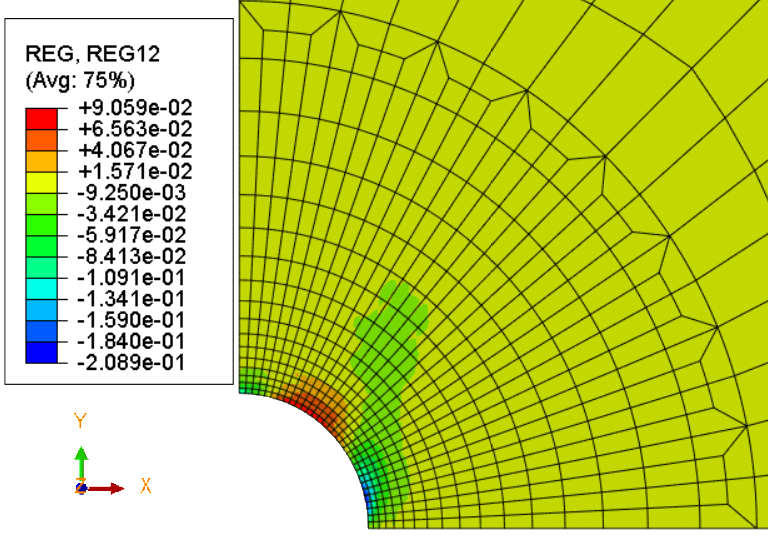
\includegraphics[scale=0.9]{Reg12_crop.png} 
	\end{center}  
   \caption{Visualization of Strain Gradient $\eta_{222} $}
\end{figure}
\begin{figure}[H]
	\begin{center}
		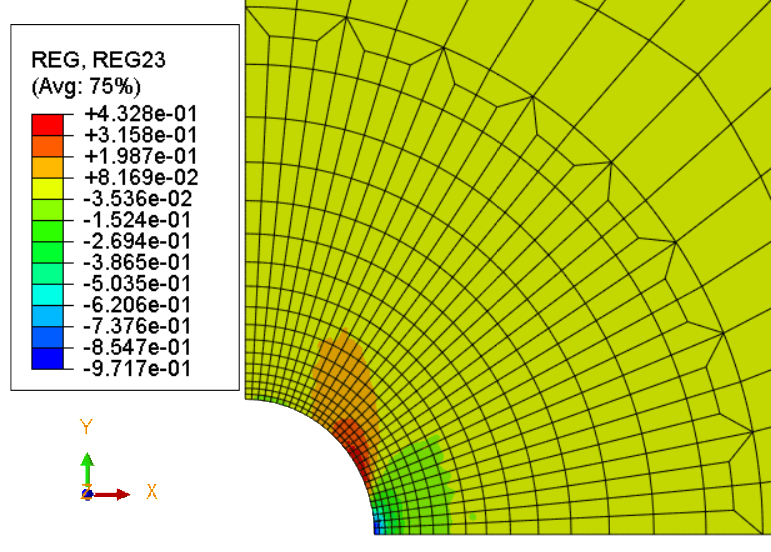
\includegraphics[scale=0.9]{Reg23_crop.png} 
	\end{center}  
   \caption{Visualization of Strain Gradient $\eta_{121}$ + $\eta_{211}$}
\end{figure}
\begin{figure}[H]
	\begin{center}
		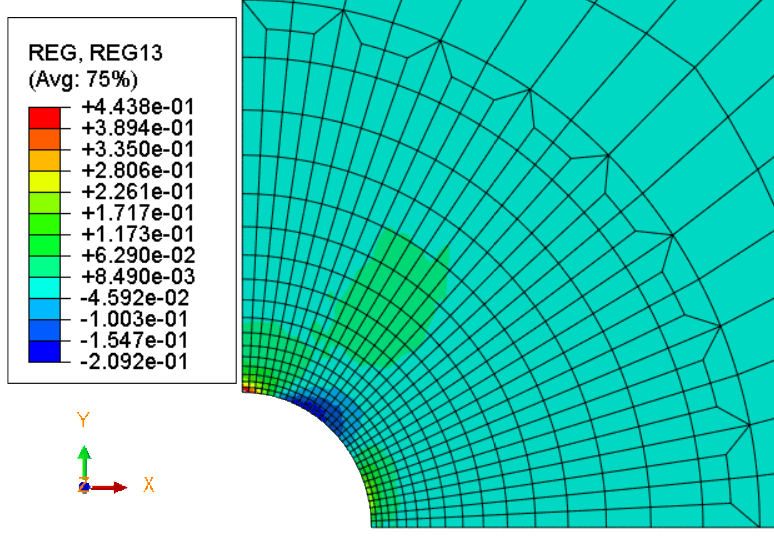
\includegraphics[scale=0.9]{Reg13_crop.png} 
	\end{center}  
   \caption{Visualization of Strain Gradient $\eta_{122}$ + $\eta_{212}$}
\end{figure}
\begin{figure}[H]
	\begin{center}
		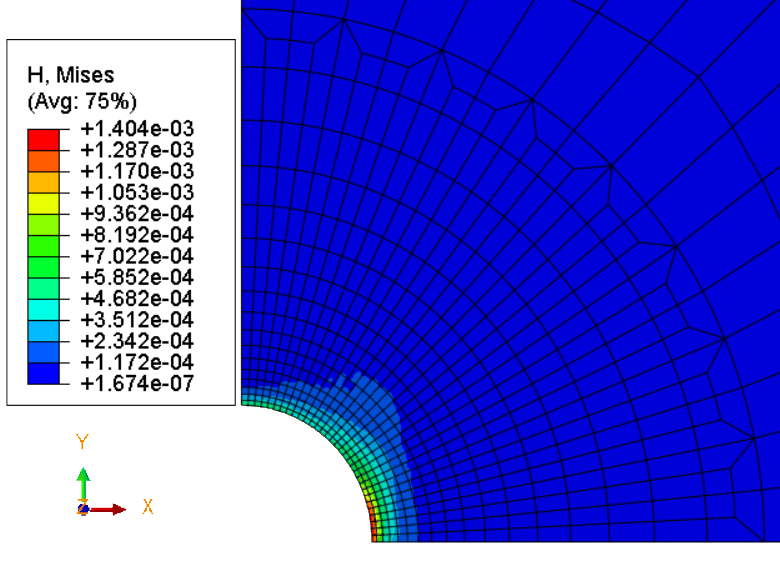
\includegraphics[scale=0.9]{Higher_order_stress_crop.png} 
	\end{center}  
	\caption{Visualization of Higher order stress in XY plane}
\end{figure}
\begin{figure}[H]
	\begin{center}
		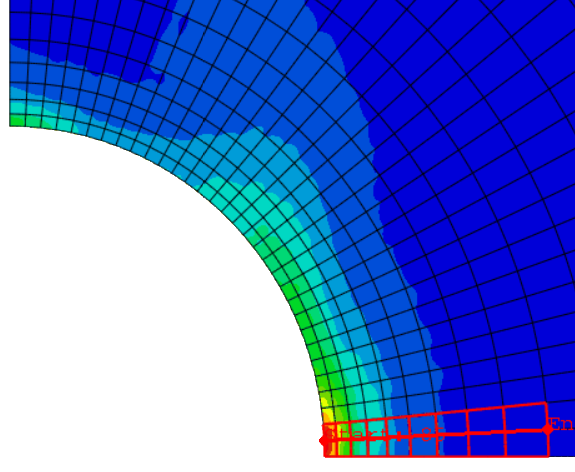
\includegraphics[scale=1]{path_full_grad_crop.png} 
	\end{center}  
	\caption{Visualization of Strain Gradient in specific path}
\end{figure}
\textbf{Strain Gradient values vs True distance along path plot:}
\begin{figure}[H]
\advance\leftskip-0.5cm
		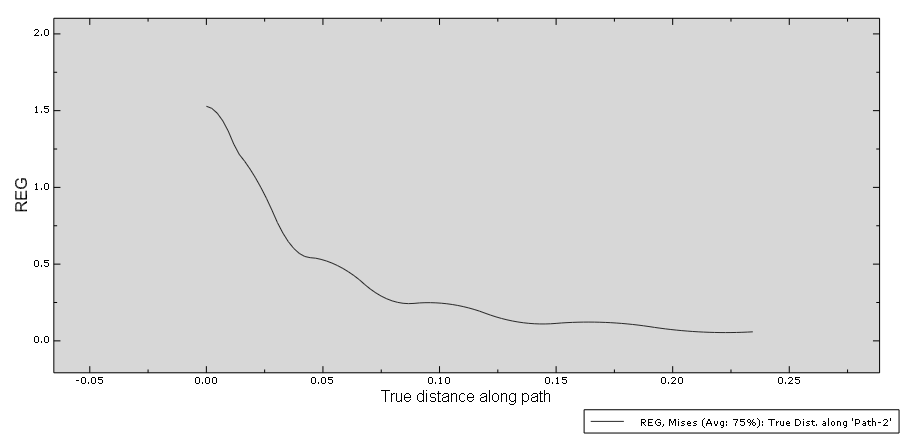
\includegraphics[scale=0.6]{path_full_grad_plot.png} 
	    \caption{Strain Gradient plot in perticular path}
\end{figure}
\vspace{1cm}
\textbf{Higher Order Stress values vs True distance along path plot:}
\begin{figure}[H]
\advance\leftskip-0.5cm
		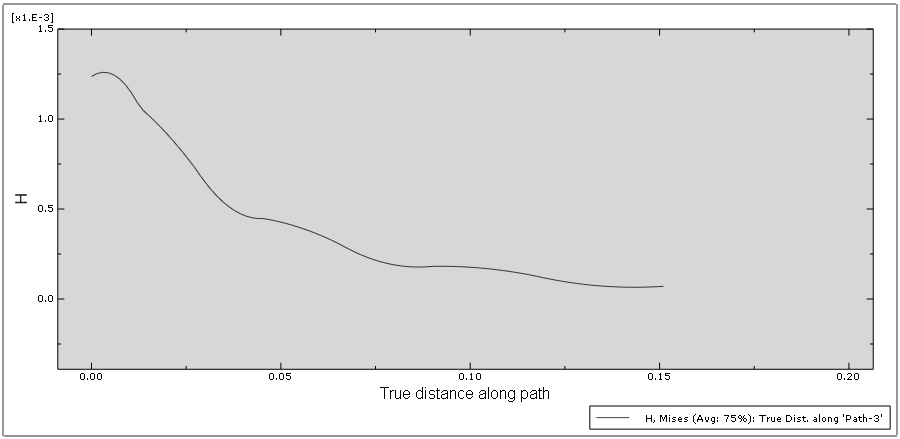
\includegraphics[scale=0.6]{Higher_order_stress_plot.png}  
	\caption{Higher order stress plot in perticular path}
\end{figure}
\newpage
As shown in above figs, the path is selected on fine mesh part to plot the Strain Gradient values along that path. In addition to that higher order stress values are also ploted on that path in below second plot. In this two plots we can see that the Higher order stress values and Strain Gradient values are getting decreasses when it goes to far from hole edge which shows the size effects. Under this loading condition (just 1$\%$ displacements of the upper edge nodes in Y-direction i.e. along the vertical edge of this model as shown in fig.) the strain gradient and Higher order stresses are not developed in simple geometry which shows clearly that the hole in the plate is very critical part and bacuase of size effect the strain gradient is generated near the hole region and this effect is decreases as going far from this region.
\\
\\
\textbf{Conclusion :} \\
\\
In this \textbf{P}ersonal \textbf{P}rogramming \textbf{P}roject(\textbf{PPP}), the Strain Gradient Elasticity theory (SGET) is implemented in FEM. The mixed FEM formulation is used to implement this model in FEM. To implement this User Element routine(UEL) is written for QU34L4 element. In addition to that two User Material routine(UMAT) for two different Strain gradient material is also written. This code is written such way that any two-dimensional complex model can simulate for strain gradient theory even for any number element mesh. From the simulation of Plate-720 with two different UMAT, it is concluded that this theory is totaly dependent on micro structural length($ l $), since for both UMAT this model is converged at different ($ l $). However this model is not converged at ($ l $) equal to the hole size, which might showing wrong results since it has to converged for same. \\
\\
This 2D code for UEL is also extended for 3D model. In this same thoery is implemented for three-dimensional model. In this the brick element BR153L9 is used, which is the straight forward extension of QU34L4 langrange element. This code is first checked by the rigid body translation test and it showing the same results as abaqus. However, this 3D code is not working for specific loading condition because of some error in code. 



\newpage
\section{Validation Tests}
In this chapter I present the Patch test which is implemented with the one element and four element of same geometry using finite element method. The Patch tests are necessary for checking the stability of the newly developed user element and also important to check the convergence of the finite element solutions.  

\subsection{Patch Test - 1}
Now, we considered an one Square geometry with specific dimensions as given below. In below given fig L = 1.0 and so therefore the coordinates of the points A(0,0), B(1,0), C(1,1) and D(0,1).  
\begin{figure}[H]
	\begin{center}
		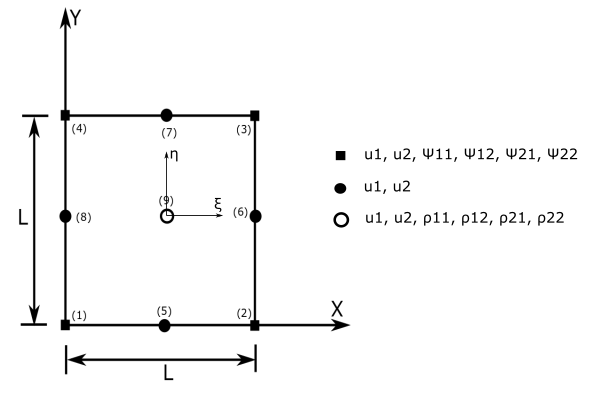
\includegraphics[scale=0.8]{ele_1.png} 
	\end{center}  
   \caption{Square Domain with one element for implementation of Patch Test-1.}
\end{figure} 
In this Patch test we just find the analytical solution for displacements and relaxed strain.
After that we are finding the values of the displacements and relaxed strain at each nodes and each corner nodes respectively by assigning the position of that node. In the last we implement the all nodal degrees of freedom in terms of the boundary condition and we find the stiffness matrix and right hand side matrix for one element by running the code with ABAQUS and we try to prove the equilibrium equation.
\\
\\
The analytical equation to find the stress,Higher order stress,displacements and relaxed strains are,
\begin{equation}\label{p_sigma}
	\sigma_{ik} = \lambda \delta_{ik} \varepsilon_{nn} + 2 \mu \varepsilon_{ik}
\end{equation}
\begin{equation}
	\tau_{jik} = \mu l^2 (u_{k,ij}- u_{j,ki}) , \qquad \tau_{lmn} = \mu l^2 (\eta_{lmn} + \eta_{nml})	
\end{equation}
\begin{equation}\label{p_psi}
	\begin{aligned}
		\psi_{11} &= u_{1,1} = -0.01x_1, \\
		\psi_{21} &= u_{1,2} =  0.02x_2, \\
		\psi_{12} &= u_{2,1} = -0.02x_1, \\
		\psi_{22} &= u_{2,2} =  0.01x_2 
	\end{aligned}
\end{equation}
\begin{equation}
	\begin{aligned}
		u_1 &= -0.005x_1^2 + 0.01x_2^2, \\
		u_2 &= -0.01x_1^2 + 0.005x_2^2,
	\end{aligned}
\end{equation}
For more details of analytical prove of above equations are given in this \cite{Lzybell2007}.
In details, we have total 18 displacements values of all nodes and 16 relaxed strain values of each corner nodes of the element which are prescribe in the Input file for one element in terms of boundary condition.  
\\ 
\\
For proving the equilibrium equation, we have stiffness matrix, RHS matrix and displacement matrix in hand. But the dimension of the above matrices are big so we wouldn't prefer to solve it on paper by hand. so i write one python scripts which reads the data of all matrices from individual files. So for that now we have to put the stiffness matrix into 'AMATRX.dat', RHS matrix into 'RHS.dat' and displacement matrix into 'U.dat' file respectively. This python file read the data and store it in terms of multidimensional array and that try to find the residual of the equilibrium equation and print it into terminal so we can verify our results. The residual from the above equilibrium equation is around 1e-07, which is almost zero compare to the stiffness matrix and rhs vector values. The more details of implementation of this test is given in "README-2D-Patch-Test-1" file.
\begin{figure}[H]
	\begin{center}
		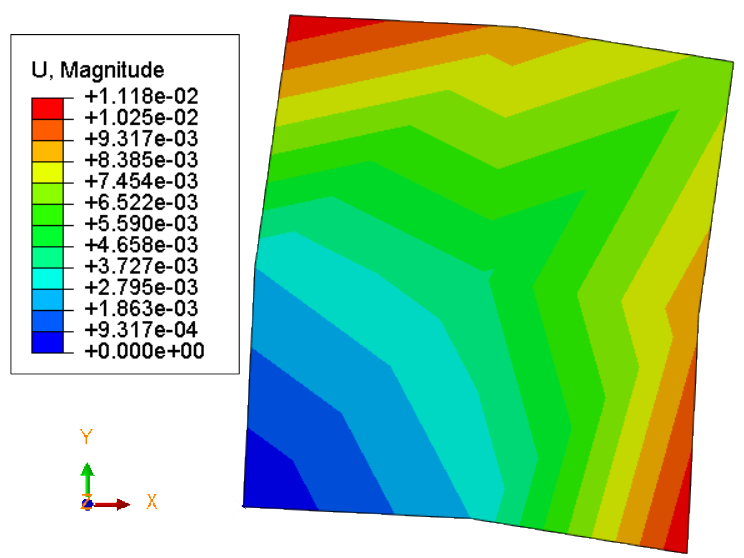
\includegraphics[scale=0.83]{patch_1_disp_crop.png} 
	\end{center}  
    \caption{Visualization of Displacement $u_1 $ in Patch Test-1 Model.}
\end{figure}
\begin{figure}[H]
	\begin{center}
		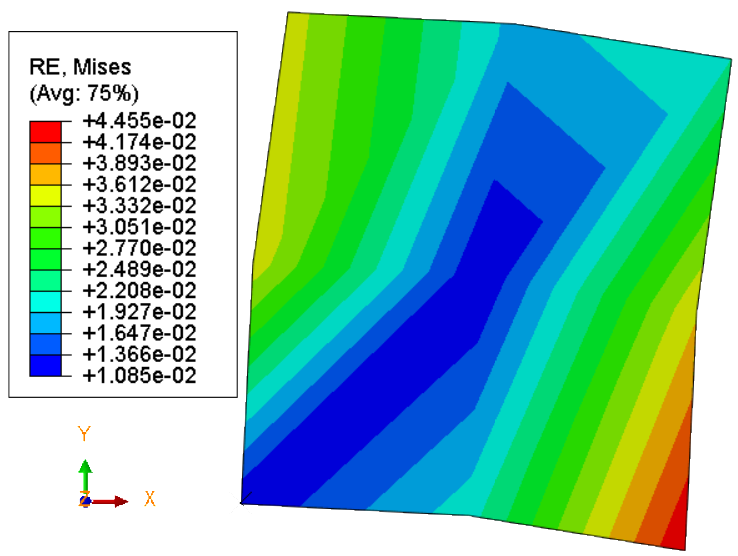
\includegraphics[scale=0.83]{patch_1_relaxed_strain_crop.png} 
	\end{center}  
    \caption{Visualization of Relaxed Strain $\psi$ in Patch Test-1 Model.}
\end{figure}
\begin{table}[H]
\begin{center}
	\begin{tabular}{||c c c c c c c||} 
		\hline
		Node Number & U1 & U2 & $\psi_{11}$ & $\psi_{12}$ & $\psi_{21}$ & $\psi_{22}$\\ [0.8ex] 
		\hline\hline
		1 & 0.0 & 0.0 & 0.0 & 0.0 & 0.0 & 0.0  \\ 
		[0.8ex]
		\hline
		2 & -0.005 & -0.01 & -0.01 & 0.0 & -0.02 & 0.0  \\ 
		[0.8ex]
		\hline
		3 & 0.005 & -0.005 & -0.01 & 0.02 & -0.02 & 0.01  \\ 
		[0.8ex]
		\hline
		4 & 0.01 & 0.005 & 0.0 & 0.02 & 0.0 & 0.01  \\ 
		[0.8ex]
		\hline
		5 & -0.00125 & -0.0025 & - & - & - & -  \\ 
		[0.8ex]
		\hline
		6 & -0.0025 & -0.00875 & - & - & - & - \\ 
		[0.8ex]
		\hline
		7 & 0.00875 & 0.0025 & - & - & - & - \\ 
		[0.8ex]
		\hline
		8 & 0.0025 & 0.00125 & - & - & - & - \\ 
		[0.8ex]
		\hline		
		9 & 0.00125 & -0.00125 & - & - & - & -\\  [0.8ex] 
		\hline
	\end{tabular}
	\caption{Input displacement and Relaxed strain values}
\end{center}
\end{table}
\newpage
\subsection{Patch Test - 2}
Now, we considered the same geometry with same dimensions as described in Patch test-1, but now we mesh it into four element as shown in below fig.
\begin{figure}[H]
	\begin{center}
		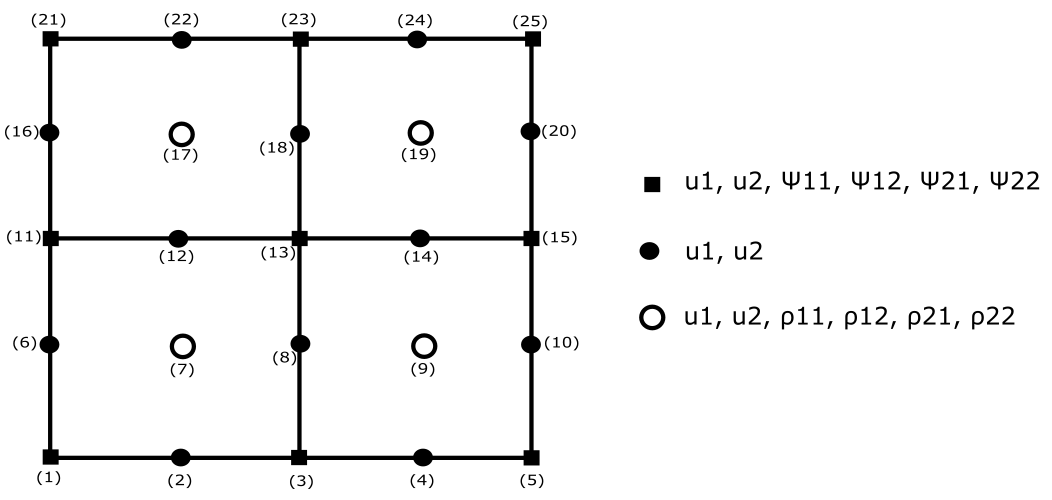
\includegraphics[scale=0.75]{ele_4.png} 
	\end{center}  
    \caption{Square Domain with four element for implementation of Patch Test-2.}
\end{figure}
Now,we trying to implement the Patch test-2, for this one there are some criteria to pass the count test therefore, we considered the four element on the same geometry instead of one. In this patch test we just find the displacements and relaxed strain of the nodes at the boundary by analytical way as same as in patch test one. 
\\
\\
In details, we have total 32 displacements values of all nodes and 32 relaxed strains values at each corner nodes of the elements which are prescribed in the Input file for four element in terms of boundary conditions.
\\
\\
As same as in Patch Test-1 i wrote the one python script for patch test-2 which also gives the analytical values of displacements and relaxed strains of the deformed nodes. we just give the values of it at the boundary and we compare the values of all inner nodes with analytical solutions. 
\\ \\
Now, we compare the Stress and Higher order stress at Gauss integration points with analytical solutions. \\ \\
Here, below data is shown the stress values ($\sigma_{11},\sigma_{22},\sigma_{12}$) at each integration points (9 integration points).
\begin{verbatim}
Stress(sigma) :

sigma(11)     -0.9355E-03 -0.4126E-02 -0.3702E-02 -0.1105E-02 -0.2531E-02 
              -0.3541E-02 -0.2403E-02 -0.1541E-02 -0.2541E-02
 
Sigma(22)      0.9355E-03  0.1105E-02  0.3702E-02  0.4126E-02  0.1541E-02  
               0.2403E-02  0.3541E-02  0.2531E-02  0.2541E-02

Sigma(12)      0.4166E-09 -0.2149E-02  0.4959E-08  0.2149E-02 -0.1205E-02 
              -0.1168E-02  0.1168E-02  0.1205E-02 -0.6108E-09
\end{verbatim}
we know the analytical equation (\ref{p_sigma}) to find the stress values at each integration points.
Here I found the analytical stress at integration point 9, which is the centre point of element 1 as shown in above fig, which coardinates is (0.25,0.25) mm. \\ \\
$\sigma_{11}$ = 2$\mu\varepsilon_{11}$ (because $\lambda$ = 0) = 2 $\dfrac{E}{2}\varepsilon_{11}$ (because $\mu = \dfrac{E}{2}$) = $\varepsilon_{11}$ (because E = 1) \\ \\
so, $\sigma_{11}$ = $\varepsilon_{11}$ = $u_{1,1}$ = $-0.01x_1$  and $\sigma_{22}$ = $\varepsilon_{22}$ = $u_{2,2}$ = $0.01x_2$ --\ref{p_psi} \\ \\
so, $\sigma_{11}$ = -0.01$\times$0.25 = -0.2500E-02 $\approx$ -0.2541E-02 \\
    $\sigma_{22}$ = 0.01$\times$0.25 = 0.2500E-02 $\approx$ 0.2541E-02 .
\begin{verbatim}

Higher Order Stress(Tau) :

Tau(111)      -0.1000E-01 -0.1000E-01 -0.1000E-01 -0.1000E-01 -0.1000E-01 
              -0.1000E-01 -0.1000E-01 -0.1000E-01 -0.1000E-01
              
Tau(221)       0.1000E-01  0.1000E-01  0.1000E-01  0.1000E-01  0.1000E-01  
               0.1000E-01  0.1000E-01  0.1000E-01  0.1000E-01
               
Tau(112)      -0.1000E-01 -0.1000E-01 -0.1000E-01 -0.1000E-01 -0.1000E-01 
              -0.1000E-01 -0.1000E-01 -0.1000E-01 -0.1000E-01
              
Tau(222)       0.1000E-01  0.1000E-01  0.1000E-01  0.1000E-01  0.1000E-01  
               0.1000E-01  0.1000E-01  0.1000E-01  0.1000E-01
               
Tau(121+211)  -0.5000E-02 -0.5000E-02 -0.5000E-02 -0.5000E-02 -0.5000E-02 
              -0.5000E-02 -0.5000E-02 -0.5000E-02 -0.5000E-02
              
Tau(122+212)   0.5000E-02  0.5000E-02  0.5000E-02  0.5000E-02  0.5000E-02  
               0.5000E-02  0.5000E-02  0.5000E-02  0.5000E-02
               
\end{verbatim}
Now, the analytical equation for Higher order stress is given below, ----\ref{p_psi}\\
$\tau_{111} = \mu l^2 (\eta_{111} + \eta_{111}) = \psi_{11,1} = -0.01$  (because $\mu = \dfrac{E}{2} and E=1,l=1$ ) \\ 
$\tau_{222} = \psi_{22,2} = 0.01$    \\
$\tau_{221} = \mu l^2 (\eta_{221} + \eta_{122}) = \dfrac{1}{2}(u_{1,22}) = 0.01$ \\
$\tau_{112} = \mu l^2 (\eta_{112} + \eta_{211}) = \dfrac{1}{2}(u_{2,11}) = -0.01$ \\
$\tau_{121+211} = \tau_{211} = \mu l^2 (\eta_{211} + \eta_{112}) = \dfrac{1}{2}(u_{2,11}) = -0.005$ \\
$\tau_{122+212} = \tau_{122} = \mu l^2 (\eta_{122} + \eta_{221}) = \dfrac{1}{2}(u_{1,22}) = 0.005$ \\ \\
So, it is conclude that Patch Test-2 for four element is also pass. The relaxed strain and Higher order Stress values are exactly match with analytical solution with error 0$\%$, whereas the displacement and Stress values are not exactly match, but the error is not bigger than 7$\%$.





\begin{table}[H]

		\begin{tabular}{||c c c c c c c||} 
			\hline
			Node Number & U1 Input& U1 Output  & U1 Expected & U2 & U2 Output & U2 Expected\\ [0.8ex] 
			\hline\hline
			1 & 0.0 & 0.0 & 0.0 & 0.0 & 0.0 & 0.0  \\ 
			[0.8ex]
			\hline
			2 & -0.0003125 & -0.0003125 & -0.0003125 & -0.000625 & -0.000625 & -0.000625  \\ 
			[0.8ex]
			\hline
			3 & -0.00125 & -0.00125 & -0.00125 & 0.02 & 0.02 & 0.02  \\ 
			[0.8ex]
			\hline
			4 & -0.0028125 & -0.0028125 & -0.0028125 & -0.005625 & -0.005625 & -0.005625  \\ 
			[0.8ex]
			\hline
			5 & -0.005 & -0.005 & -0.005 & -0.01 & -0.01 & -0.01 \\ 
			[0.8ex]
			\hline
			6 & 0.000625 & 0.000625 & 0.000625 & 0.0003125 & 0.0003125 & 0.0003125 \\ 
			[0.8ex]
			\hline
			\rowcolor{lightgray} 7 & - & 0.0001510 & 0.0003125 & - & -0.0001510 & -0.0003125 \\ 
			[0.8ex]
			\hline
			\rowcolor{lightgray} 8 & - & -0.000645 & -0.000625 & - & -0.0021668 & -0.0021875 \\ 
			[0.8ex]
			\hline	
			\rowcolor{lightgray} 9 & - & -0.0023437 & -0.0021875 & - & -0.0051562 & -0.0053125  \\ 
			[0.8ex]
			\hline
			10 & -0.004375 & -0.004375 & -0.004375 & -0.0096875 & -0.0096875 & -0.0096875  \\ 
			[0.8ex]
			\hline
			11 & 0.0025 & 0.0025 & 0.0025 & 0.00125 & 0.00125 & 0.00125  \\ 
			[0.8ex]
			\hline
			\rowcolor{lightgray} 12 & - & 0.0021668 & 0.0021875 & - & 0.000645 & 0.000625  \\ 
			[0.8ex]
			\hline
			\rowcolor{lightgray} 13 & - & 0.00133 & -0.00125 & - & -0.00133 & -0.00125  \\ 
			[0.8ex]
			\hline
			\rowcolor{lightgray} 14 & - & -0.0003331 & -0.0003125 & - & -0.004354 & -0.004375 \\ 
			[0.8ex]
			\hline
			15 & -0.0025 & -0.0025 & -0.0025 & -0.00875 & -0.00875 & -0.00875 \\ 
			[0.8ex]	
			\hline
			16 & 0.005625 & 0.005625 & 0.005625 & 0.0028125 & 0.0028125 & 0.0028125 \\ 
			[0.8ex]
			\hline	
			\rowcolor{lightgray} 17 & - & 0.0051562 & 0.0053125 & - & 0.0023437 & 0.0021875  \\ 
			[0.8ex]
			\hline 
			
			\rowcolor{lightgray} 18 & - & 0.004354 & 0.004375 & - & 0.0003331 & 0.0003125 \\ 
			[0.8ex]
			\hline
			\rowcolor{lightgray} 19 & - & 0.0026510 & 0.0028125 & - & -0.0026510 & -0.0028125  \\ 
			[0.8ex]
			\hline
			20 & 0.000625 & 0.000625 & 0.000625 & -0.0071875 & -0.0071875 & -0.0071875  \\ 
			[0.8ex]
			\hline
			21 & 0.01 & 0.01 & 0.01 & 0.005 & 0.005 & 0.005  \\ 
			[0.8ex]
			\hline
			22 & 0.0096875 & 0.0096875 & 0.0096875 & 0.004375 & 0.004375 & 0.004375 \\ 
			[0.8ex]
			\hline
			23 & 0.00875 & 0.00875 & 0.00875 & 0.0025 & 0.0025 & 0.0025 \\ 
			[0.8ex]
			\hline
			24 & 0.0071875 & 0.0071875 & 0.0071875 & -0.000625 & -0.000625 & -0.000625 \\ 
			[0.8ex]	
			\hline
			25 & 0.005 & 0.005 & 0.005 & -0.005 & -0.005 & -0.005 \\  [0.8ex] 
			\hline
		\end{tabular}
		\caption{Displacement Values in Patch test-2.}

\end{table}

\begin{table}[H]
	\begin{center}
		\begin{tabular}{||c c c c c||} 
			\hline
			Node Number & $\psi_{11}$ Output & $\psi_{11}$ Expected  & $\psi_{22}$ Output & $\psi_{22}$ Expected \\ [0.8ex] 
			\hline\hline
			1 & 0.0 & 0.0 & 0.0 & 0.0  \\ 
			[0.8ex]
			\hline
			3 & -0.005 & -0.005 & 0.0 & 0.0  \\ 
			[0.8ex]
			\hline
			5 & -0.01 & -0.01 & 0.0 & 0.0   \\ 
			[0.8ex]
			\hline
			11 & 0.0 & 0.0 & 0.005 & 0.005   \\ 
			[0.8ex]
			\hline
			\rowcolor{lightgray} 13 & -0.005 & -0.005 & 0.005 & 0.005  \\ 
			[0.8ex]
			\hline
			15 & -0.01 & -0.01 & 0.005 & 0.005  \\ 
			[0.8ex]
			\hline
			21 & 0.0 & 0.0 & 0.01 & 0.01  \\ 
			[0.8ex]
			\hline
			23 & -0.005 & -0.005 & 0.01 & 0.01  \\ 
			[0.8ex]
			\hline	
			25 & -0.01 & -0.01 & 0.01 & 0.01   \\ 
			[0.8ex]
			\hline
		\end{tabular}
		\caption{Relaxed Strain $\psi_{11}$ and $\psi_{22}$ Values in Patch test-2.}
	\end{center}
\end{table}

\begin{table}[H]
	\begin{center}
		\begin{tabular}{||c c c c c||} 
			\hline
			Node Number & $\psi_{21}$ Output & $\psi_{21}$ Expected  & $\psi_{12}$ Output & $\psi_{12}$ Expected \\ [0.8ex] 
			\hline\hline
			1 & 0.0 & 0.0 & 0.0 & 0.0  \\ 
			[0.8ex]
			\hline
			3 & 0.0 & 0.0 & -0.01 & -0.01  \\ 
			[0.8ex]
			\hline
			5 & 0.0 & 0.0 & -0.02 & -0.02   \\ 
			[0.8ex]
			\hline
			11 & 0.01 & 0.01 & 0.0 & 0.0   \\ 
			[0.8ex]
			\hline	
			\rowcolor{lightgray} 13 & 0.01 & 0.01 & -0.01 & -0.01  \\ 
			[0.8ex]
			\hline
			15 & 0.01 & 0.01 & -0.02 & -0.02  \\ 
			[0.8ex]
			\hline
			21 & 0.02 & 0.02 & 0.0 & 0.0  \\ 
			[0.8ex]
			\hline
			23 & 0.02 & 0.02 & -0.01 & -0.01  \\ 
			[0.8ex]
			\hline	
			25 & 0.02 & 0.02 & -0.02 & -0.02   \\ 
			[0.8ex]
			\hline
		\end{tabular}
		\caption{Relaxed Strain $\psi_{21}$ and $\psi_{12}$ Values in Patch test-2.}
	\end{center}
\end{table}

\subsection{Rigid Body Translation Test}
\vspace{1cm}
\begin{figure}[H]
	\begin{center}
		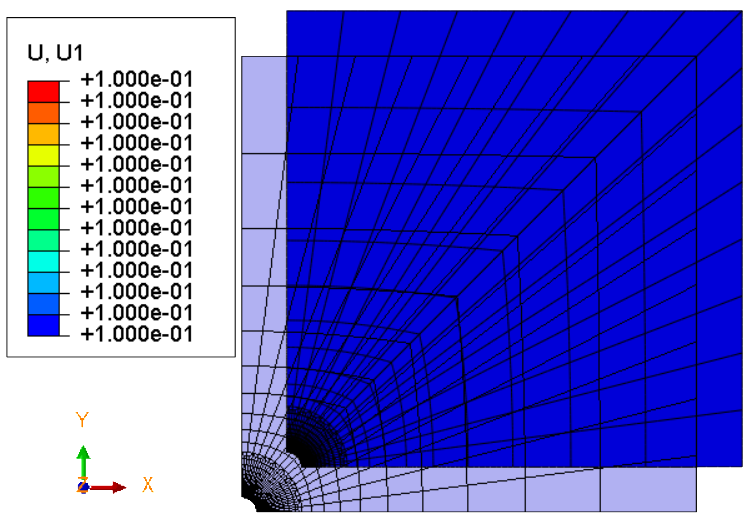
\includegraphics[scale=0.49]{Rigid_body_u1_crop.png} 
	    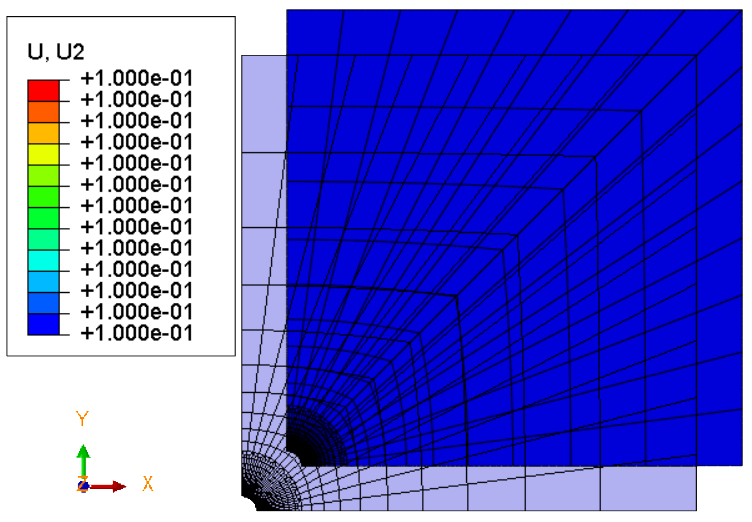
\includegraphics[scale=0.49]{Rigid_body_u2_crop.png} 
	\end{center}
	\caption{Visualization of Displacement $u_1 $ and $u_2 $ in Rigid Body Transformation Test.} 
\end{figure}
\vspace{1cm}
\begin{figure}[H]
	\begin{center}
		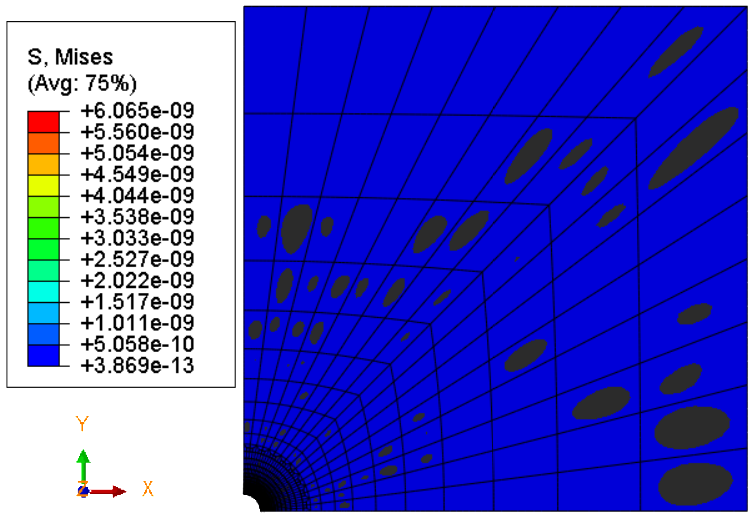
\includegraphics[scale=0.49]{Rigid_body_stress_crop.png} 
		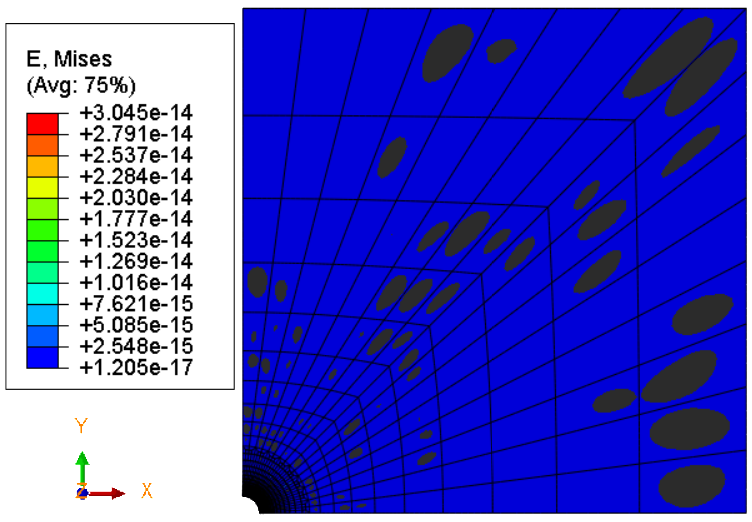
\includegraphics[scale=0.49]{Rigid_body_strain_crop.png} 
	\end{center}
	\caption{Visualization of stress and strain in Rigid Body Transformation Test.} 
\end{figure}
\vspace{1cm}
In this "Rigid Body Translation" test, I gave the displacements to the uper edge nodes in positive X and Y direction equals to the 0.1mm. So there is no boundary condition, therfore the geometry moves rigidly and there is no reaction forces at any nodes. Due to this there is no stress and strain emerges into the elements. Above both figures shown the displacements, Stresses and Strains into the Plate-720 geometry after the Rigid body translation test. For more information on how to implement this test is given in "README-2D-Rigid-Body-Translation" file.
\newpage
\section{Documentation of the Programming work}
\subsection{Implementation details of FEM model}
In this section, the brief overview of implementation details of FEM model plate-720 is given.
\subsubsection{ Preprocessing}
\begin{itemize}
	\item In plate-720 model there is total 720 element as shown in fig.
	\item I mesh the $10\times10$ mm square plate with circular hole of radius 0.333 mm as shown in fig, with ABAQUS element CPS8, using the transition of mesh from fine to coarse mesh.
	\item The transition of mesh is occured at the distance 1.332 mm from the centre of the hole. For more details see the section "Verification  of model plate-720".
	\item One Python code is written, which convert this 8-noded element(CPS8) mesh into 9-noded element(QU34L4) mesh by including the centre node in each element.
	\item After getting this new nodes and elements data are used in new Input file for plate-720, which is simulating with UEL.
\end{itemize}
\subsubsection{ Processing}
The main task in Processing is to develope user element routine(UEL) for QU34L4 element to implement the strain gradient elsticity theory.

\begin{itemize}
	\item \textbf{Input-Output Parameters.} \\
	\\
	In UEL subroutine for ABAQUS there is one standard format to defined the input and output parameters. Even there are some standaerd variables which are predefined in ABAQUS. So, it has to be used to developed the UEL. The input parameters to the UEL like material property, coordinates and displacement of nodes, external load to the model. Outputs are amatrx-stiffness matrix and rhs-force vector mainly.
	\\
	\item \textbf{Initialization and Dimensioning of the Arrays.} \\
	\\
	In fortran programming language it is mandetory to initialize and give dimension to every arrays whether it is vector or matrix. There is another one best practice in fortran is to giving the double precision to the every scalar parameters also. In fortran "dimension() ::" is used to give dimension and "parameter" is used to defined the scalar parameters with it fixed values. To define the array with its predifined values the "data" is used.		
\end{itemize}

\begin{table}[H]
	\begin{center}
		\begin{tabular}{||c ||} 
			\hline
			\textbf{Start UEL} \\ [0.8ex] 
			\hline\hline
			Input Parameters, Output Parameters  \\ 
			[0.8ex]
			\hline
			Initialization of all arrays  \\ 
			[0.8ex]
			\hline
		    Dimensioning of all arrays  \\ 
			[0.8ex]
			\hline
			\textbf{CALL} Shape function subroutine for displacement \\ 
			[0.8ex]
			\hline
			\textbf{CALL} Shape function subroutine for relaxed strain   \\ 
			[0.8ex]
			\hline
			\textbf{CALL} Jacobian subroutine for displacement \\ 
			[0.8ex]
			\hline
			\textbf{CALL} Jacobian subroutine for relaxed strain  \\ 
			[0.8ex]
			\hline
			\textbf{CALL} B-Matrix subroutine for displacement  \\ 
			\hline
			\textbf{CALL} B-Matrix subroutine for relaxed strain  \\ 
			[0.8ex]
			\hline		
			\textbf{Assembly of the following Matrices :} \\
			1) Shape-Matrix for displacement DOF \\
			2) Displacement-Gradient-Matrix \\
			3) B-Matrix \\
			4) Shape-Matrix for Relaxed-Strain DOF \\
			5) B-Matrix for Relaxed-Strain DOF \\
			6) Shape-Matrix for Lagrange-Multiplier DOF \\
			[0.8ex] 
			\hline
			\textbf{State Variables} Calculations   \\  [0.8ex] 
			\hline
			\textbf{CALL} UMAT - material subroutine   \\  [0.8ex] 
			\hline
			\textbf{Stiffness Matrices} Calculations  \\  
			1) $K_{UU}$ \\
			2) $K_{PsiPsi}$ \\
			3) $K_{Urho}$ \\
			4) $K_{Psirho}$ \\   [0.8ex] 
			\hline
			\textbf{Internal Force Vectors} Calculations  \\  [0.8ex] 
			\hline
			\textbf{Assembly of Global Stiffness Matrix and RHS vector}   \\  [0.8ex] 
			\hline
			\hline
		    \textbf{End UEL}   \\  [0.8ex] 
		    \hline
		\end{tabular}
		\caption{Implementation flow of UEL}
	\end{center}
\end{table}

\begin{itemize}
	\item \textbf{Shape Function Subroutine.} \\
	In this UEL for QU34L4 element there are two types of shpe function are used. One is standard quadratic shape function to interpolate the displacement DOF and the second is standard bi-linear shape function to interpolate the newly introduced DOF relaxed strain. In both subroutine this two shape functions and their derivatives with respect to two area-coordinates $\xi$ and $\omega$ respectively defined. In addition to that the Gauss point coordinated are also defined which are the input to this shape functions and their derivatives. \\
	\\
	\textbf{Input} : current integration point \\
	\textbf{Output} : Shape-Function-Matrix, differentiation of Shape-Function-Matrix
	\\
	\\
	\item \textbf{Jacobian Matrix Subroutine.} \\
	As of seen in Shape function subroutine there are total two types of shape functions so for that two Jacobian matrix are defined in this subroutine. Along with the Jacobian matrix the "Determinant" and "Inverse" of Jacobian matrix are also determind in this subroutine. \\ \\
	\textbf{Input} : current element number, coordinates of all nodes of current element, \qquad  differentiation of Shape-Function-Matrix \\
	\textbf{Output} : Determinant of Jacobian matrix, Inverse Jacobian matrix

	\item \textbf{B-Matrix Subroutine.} \\
	In this subroutine the differential matrix for shape function derivatives are arranged.
	Therefore, the inverse Jacobian matrix from Jacobian Matrix subroutine and differentiation of shape function from Shape function subroutine are used as input in this subroutine. \\ \\
	\textbf{Input} : Inverse Jacobian matrix, differentiation of Shape-Function-Matrix  \\
	\textbf{Output} : B-Matrix(differential Matrix)
	
	\item \textbf{Assembly of Common Matrices.} \\
	Now from the above three subroutines, we got the suffiecient data to assemble the necessary martices to find the state variables and element matrices. In this section of code following matrices are determined, \\ \\
	N-Matrix(shape function matrix related to displacement DOF) \\
	M-Matrix(differentiation of N-matrix) \\
	B-Matrix(differentiation of N-matrix but different arrangement than M-Matrix) \\
	Npsi-Matrix(shape function matrix related to relaxed strain DOF) \\
	Bpsi-Matrix(differentiation of Npsi-Matrix) \\
	Nrho-Matrix(Identity matrix)
	
	\item \textbf{Calculation of State Variables.}\\
	In this section of the code the following state variables are determinded with the help of the above determined Common Matrices and input DOF(displacements, delta-displacements, relaxed-strain, delta-relaxed-strain, langrange multiplier) values. \\ \\
	Displacement Gradient (M-matrix, displacements) \\
	Strain (B-Matrix, displacements) \\
	Delta Strain (B-Matrix, delta-displacements) \\
	Relaxed Strain (Npsi-Matrix, relaxed-strain) \\
	Relaxed Strain Gradient (Bpsi-Matrix, relaxed-strain) \\
	Delta Relaxed Strain Gradient (Bpsi-Matrix, delta-relaxed-strain) \\
	Langrange Multiplier (Nrho-Matrix, langrange-multiplier)
	
	\item \textbf{UMAT - User Material Subroutine} \\
	In this subroutine another two state variables "Stress" and "Higher order stress" are determined. In this subroutine the elastic matrix(which connects stress and strain) and Higher order elastic matrix(which connects higher order stress and relaxed strain gradient) are also defined. The Higher order elastic matrix is determined for two different type of strain geadient material. The most intersting conclusion of these two UMAT is that they both give approximately same results at microstructural length($l$) 0.0001 mm. However, they do not converge at same $l$. One is only converged at min $l$ at 0.0001 mm and second even converge at 0.01 mm $l$. \\ \\
	\textbf{Input} : Lemda, Mue (lame constant)  \\
	Microstructural length (Material Property) \\
	Current Integration Point \\
	Strain, Relaxed strain gradient (state variables) \\
	\textbf{Output} : C-Matrix, D-Matrix (Elastic and Higher order elastic matrix resp.) \\
	Sigma, Tau (Stress and Higher order stress - State variables)
	
	\item \textbf{Calculation of Stiffness Matrices}
	In this section of code, the Stiffness Matrix related to individual DOF are found. There are total four stiffness matrix to find, \\ \\
	$K_{UU}$ - Stiffness Matrix related to only displacement DOF (Dimesndion $18\times18$)
	$K_{PsiPsi}$ - Stiffness Matrix related to only relaxed-strain DOF (Dimesndion $16\times16$)
	$K_{Urho}$ - Stiffness Matrix related to displacement and langrange multiplier DOFs (Dimesndion $18\times4$) \\
	$K_{Psirho}$ - Stiffness Matrix related to relaxed-strain and langrange multiplier DOFs (Dimesndion $16\times4$)
	
	\item \textbf{Calculation of Internal Force Vectors} \\
	In this section of code, the Internal forces due to reaction of different DOFs. There are total three Internal Forces to find related three different DOFs, \\ \\
	$F_{int}$ - Internal force ralated to only displacement DOF (Dimension 18$\times$1) \\
	$R_{int}$ - Internal force ralated to only relaxed-strain DOF (Dimension 16$\times$1) \\
	$S_{int}$ - Internal force ralated to only langrange-multiplier DOF (Dimension 4$\times$1)
	
	\item \textbf{Assembly of Global Stiffness Matrix and RHS Vector} \\
	In above both section the Individual Stiffness matrices and Internal force vectors are find out, So now assembly of these into Global Stiffness Matrix and Global RHS Vectors can be done into this section of code. \\
	
	\begin{equation}\label{global_stiff}
	\textbf{K}=
	\begin{bmatrix}
	K_{UU}&0&-K_{URho} \\
	0&K_{PsiPsi}&K_{PsiRho}\\
	-K_{URho}^T&K_{PsiRho}^T&0\\
	\end{bmatrix}
	\end{equation}

	\begin{equation}\label{global_force}
	\textbf{RHS}=
	\begin{bmatrix}
	F_{int} \\
	R_{int} \\
	S_{int} \\
	\end{bmatrix}
	\end{equation}	
	
\end{itemize}



\subsubsection{ Post-Processing}
\begin{itemize}
	\item Finally, after simulating the Plate-720 with user developed element it is time to visualize the model in ABAQUS and visulaize the desired outputs. 
	\item In ABAQUS there is no 9-noded element, so to visualize the UEL we have to use the \textbf{Dr.-Ing. Stephan Roth's} tool, which is described in appendix.
	\item Do all the procedures which is described in appendix, than after it can be run with another code which is also given in appendix.
	\item After successfully run the code, the ODB file is updated with new data.
	\item Open the ODB file in ABAQUS 6.14 version.
	\item Now the deformed model is visualized with QU34L4 element.
\end{itemize}


\subsection{Problem Faced during Programming UEL}
In this section,it is mentioned the errors and problems I faced during the learning the Fortran programming language and also code this User Element in fortran programming language. 
\begin{itemize}
	\item Syntax errors in fortran which are totaly different from common programming languages like "Python" or "C".
	\item Intialization and dimensioning of all vectors and matrix and even scalar variables also. 
	\item Getting "Non Apllicable Number (NAN)" in output because of not giving proper dimensionig or intialization of any variables or input parameters.
	\item How to define the "Degree Of Freedom (DOF)" for each nodes in User element, which has not unique DOF at each nodes.
	\item While using DOF relaxed strain in UEL as number 21,22,23,24, the DOF 23 and 24 is not working while giving input values to it and gives the error "Illegal memory reference" (signal 11). However, it is working well without giving input to this DOF 23 and 24.
	\item "Distrubuted load(DLOAD)" can not directly added to the internal force vector(rhs), due to this reason the new subroutine DLOAD has to be codded for User element routine.
	\item The assembaly of global stiffness matrix(amatrx). The user element QU34L4 has total 38 DOF and it is not unique at each nodes. Therefor, there are two possible ways to defines global stiffness matrix from individual matrix related to DOF.
	\item The above problem also faced for the global rhs vector due to the same reason.
	\item Micro-Structural Length ($l$), which is input parameters as material property. The strain gradient elasticity theory is explicitly depend on it. In the starting stage of the excecution of UEL, I was getting the wrong results due to wrong selection of matrial property $l$.  
	\item There are two User material for strain gradient elasticity theory and both of them working for different microstructural length.
	\item Postprocessing of the user element QU34L4 element in commercial software ABAQUS. In abaqus there is no element which has nine node. So, for postprocessing Dr.-Ing. Stephan Roth's tool is used and dummy element CPS8 is used to visualize the QU34L4 in ABAQUS.
\end{itemize}
\subsection{Milestones achieved}
\begin{itemize}
	\item Implementation of UEL routine for strain gradient elasticity theory in fortran programming language.
    \item Comparision of classical continum theories and strain gradient elasticity theories.
    \item Implementation of FEM model based on Aifantis or Mindlin theories.
    \item Simulation of plate with circular hole (Plate-720).
    \item Validation and verification of FEM model by various numerical tests.
\end{itemize}
\textbf{Extra achieved goals :}
\begin{itemize}
	\item Postprocessing and visualization of user element with ABAQUSER.
	\item Write code for KDLOAD.
	\item Mesh Plate-720 standard geometry includes transition of mesh from fine to coarse mesh.
	\item An attempt to extend the code to 3D case as an extra activity during deadline extension.
	\item Python code to convert 8 node element mesh into 9 node element mesh.
	\item Conversion of 20 nodes element mesh into 27 nodes element mesh.
\end{itemize}
\vspace{1cm}
\textbf{Special Note :} \\
As of seen in my whole report I used the John.Y shu mixed Fem formulation and used QU34L4 element. On this topic, Lutz Zybell is also done his diplom thesis. I dont have any source related to this thoery from the starting of the coding of UEL to until now. However that diplom thesis is provided to me for the report purpose and also gaining the deep knowledge about this theory. I have also refer the paper which is published by him on this theory.

\newpage

\section{3D Model}
\subsection{3D element}
In addition to this PPP proposal, the extension of the above 2D UEL is done within this PPP duration. In this section a straightforward extension of the two-dimensional finite element QU34L4 introduce by John Y. shu et al. into the three-dimensional finite element BR153L9 is presented. 
\\
\\
\begin{figure}[H]
	\begin{center}
		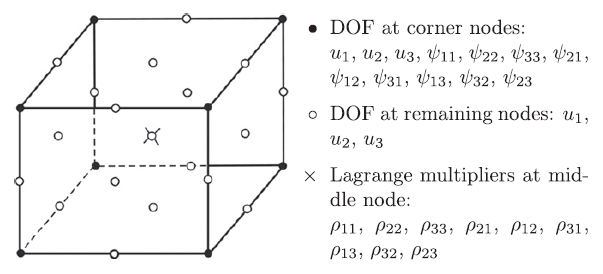
\includegraphics[scale=1.2]{3d_element.png}  
	\end{center}  
	\caption{Sketch of BR153L9 element(3D). \cite{zybell2012three}}
\end{figure}
The newly introduced isoparametric brick element BR153L9, as shown in above fig, is also known as Lagrangian finite element, because it uses nine Lagrange Multipliers $\rho_{ij}$ which are assumed to be constant throughout the element and which are connected to the centre node of the element. This element has total 27 nodes and 162 degrees of freedom(DOF). There are twelve DOF $u_i$ and $\psi_{ij}$ at each corner node and three DOF $u_i$ at each of the remaining 19 nodes. As of seen in 2D element QU34L4, the displacement and relaxed strain interpolate with different shape functions. Here, displacements $u_i$ are interpolated by the conventional tri-quadratic Langrangian shape functions and the relaxed strains $\psi_{ij}$ are interpolated tri-linearly.	\\
\\
As of discussed above this 3D element BR153L9 is ease extension of 2D element QU34L4 element, so after developing the UEL for 2D element, the 3D case is also extended. For suirity of working of this 3D element, the rigid body translation test is also done and it also give the expected results, but in later I realized that there is one error in 3D UEL, because of which it is not converged for specific loading condition.

\subsection{Rigid body translation test of 3D model.}
First we visualize the 3D model, which is mesh with 3D element BR153L9 in below fig,
\begin{figure}[H]
	\begin{center}
		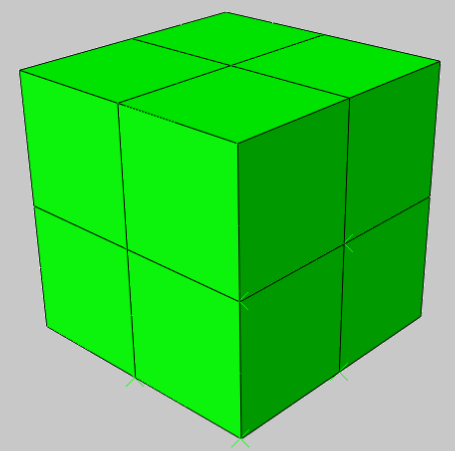
\includegraphics[scale=0.9]{3d_model_8_element_crop.png}  
	\end{center}  
	\caption{3D model mesh with 8 BR153L9.}
\end{figure}
The above 3D model dimesions are (10$ \times $10$ \times $10) mm. In this model the vertical edge is presenting the Y-direction(Y-axis). In this rigid body translation test, the only displacement boundary condition is given to the upper surface node. In this case 0.1 mm predefined displacement is given to the uppersurface along Y-direction.
\begin{figure}[H]
	\begin{center}
		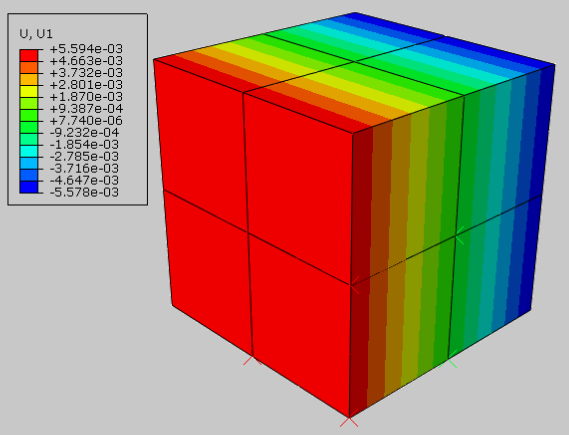
\includegraphics[scale=1.1]{3d_model_U1_crop.png}  
	\end{center}  
	\caption{Displacement of 3D model in x-direction$(u_1)$.}
\end{figure}
\begin{figure}[H]
	\begin{center}
		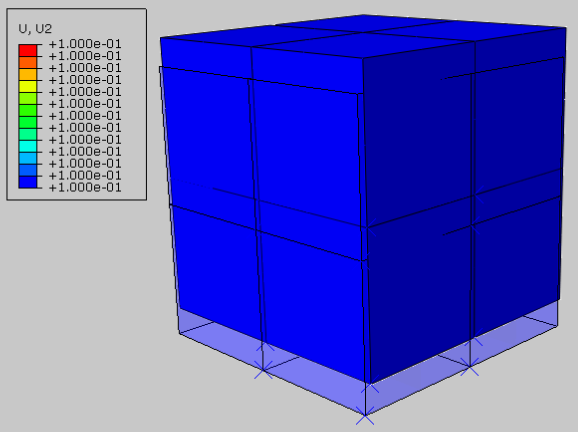
\includegraphics[scale=1.1]{3d_model_U2_crop.png}  
	\end{center}  
	\caption{Displacement of 3D model in Y-direction$(u_2)$.}
\end{figure}
\begin{figure}[H]
	\begin{center}
		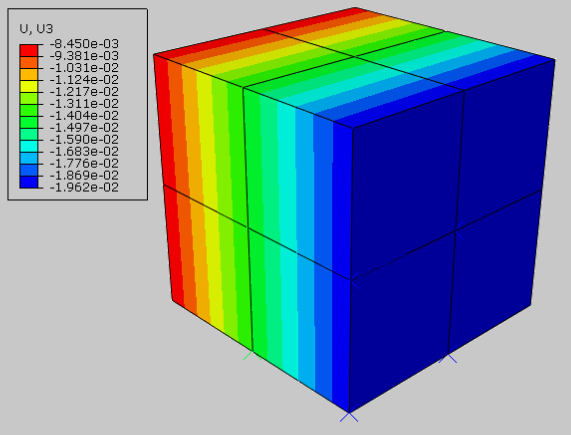
\includegraphics[scale=1.1]{3d_model_U3_crop.png}  
	\end{center}  
	\caption{Displacement of 3D model in z-direction$(u_3)$.}
\end{figure}
\begin{figure}[H]
	\begin{center}
		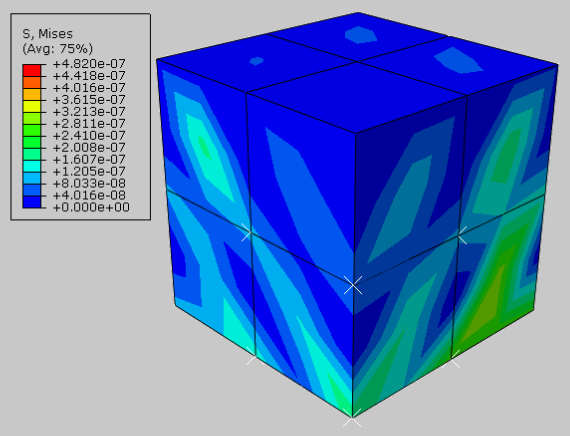
\includegraphics[scale=1]{3d_model_S_crop.png}  
	\end{center}  
	\caption{Stresses$(\sigma)$ developed in 3D model.}
\end{figure}
\begin{figure}[H]
	\begin{center}
		\includegraphics[scale=1]{3d_model_E_crop.png}  
	\end{center}  
	\caption{Strains$(\varepsilon)$ developed in 3D model.}
\end{figure}
In conclusion, it is easily seen that the displacement in Y-direction is same at each node, which shaws the rigid body translation. In addition to that there is no reaction forces because of no additional boundary condition other than the displacement in Y-direction. Therefore there is no stresses and strains developed in element.




\begin{appendices}
\section{Python file for Patch test-1}
\includegraphics[scale=0.80,page=1]{Patch_test_1_elem_eqn.pdf} 
\\
\\
\includegraphics[scale=0.80,page=1]{pro.pdf}
\section{Python file for Patch test-2}
\includegraphics[scale=0.80,page=1]{Patch_Test_4_elem_eqn.pdf}
\\
\\
\includegraphics[scale=0.80,page=2]{Patch_Test_4_elem_eqn.pdf}
\section{Python file for 9-node Element mesh generation}
\includegraphics[scale=0.80,page=1]{9Node_Mesh_generation.pdf}
\\
\\
\includegraphics[scale=0.80,page=2]{9Node_Mesh_generation.pdf}
\section{Flowchart of Strain Gradient Elasticity FEM Model}
\vspace{5cm}
\includegraphics[scale=0.60,page=1]{flow_chart_1.pdf}
\newpage
\begin{center}
	\includegraphics[scale=0.60,page=1]{flow_chart_2.pdf}
	\captionof{figure}{Flowchart of the Strain Gradient Elasticity theory FEM formulation.}
\end{center}
\newpage
\section{Postprocessing tool to visualize UEL}
We know that commercial Software ABQUS has large range of Eelements which is defined in it. We can use those elements only to visualize the any FEM model. To visualize the User defined Element and any FEM model in ABAQUS \textbf{Dr.-Ing. Stephan Roth} developed one tool. This tool helps us to postprocess any FEM model by replacing the UEL with ABAQUS defined Element.
\\
\newline
There are few steps, which I had to do for the postprocessing of UEL using the tool, are given below,
\newline
\\
\textbf{1)} First of all, the input file has to modified such that it produced one (.fil) file. There are some sequence in order to defined the different parameters in (.inp) input file, such as *part, *Assembly, *instance, *node, *user element, *Uel property, *element in sequence.
In the last part of input file it has to modified the output request according to out reuqirement in postprocessing.
\\
\\
\textbf{(2)} In second step we have write one (.info) which contains the UEL information. It can be modified according to the many different parameters such as "Degree of Freedom(DOF)", "Number of nodes per element", "Number of Guass points per element", "Number of dimension(DIM)" and finally "Number of solution dependent state variable(SDV)". In this file we have to also give the dummpy element name, which is defined in ABAQUS already, in order to get the desired property in visualization. 
\\
\\
\textbf{(3)} In third step we have to put the some of the files in same folder, in which we run the userelement routine with input file, in order to call the basic environement files for the postprocessing during call the processing code, such as (.info), (ABAQUSER.pyc), (.fil), (abaqusv6.env), and most important (.inp) and (.f) files.
\\
\\
\textbf{(4)} In the last we have to run the Ueser element routine using linux command line or Abaqus commmand prompt by following code.
\\
\\
\textbf{Code 1 : abq6142 job=$<\textbf{Input-file-name}>$ user=$<\textbf{fortran-file-name}>$}
\\
\textbf{Code 2} : \textbf{abq6142} \textbf{python} \textbf{ABAQUSER.pyc} $<\textbf{Input-file-name}>$ \\
\textbf{ABACALL=abq6142} $<\textbf{Info-file-name}>$

\newpage
\section{Git history}
\begin{verbatim}
commit c49f7b46f19fbd2b419529c54d809f761aefd4a5
Author: Dhaval Rasheshkumar Patel <dhavalrpatel2511@gmail.com>
Date:   Sat Apr 4 12:01:54 2020 +0200

Rename the Fortran file(UEl) from first_1 to UEL_2D.

commit 27aabe75271e3a27c4205f933002e8f157536307
Author: Dhaval Rasheshkumar Patel <dhavalrpatel2511@gmail.com>
Date:   Sat Apr 4 12:00:00 2020 +0200

After add the final comments and whole details of each specific 
subroutine and sections.

commit 9dfb334fc054b781d24b8765e5cbb2be556c9ede
Author: Dhaval Rasheshkumar Patel <dhavalrpatel2511@gmail.com>
Date:   Thu Mar 26 18:40:16 2020 +0100

Finalized code after adding the second gradient material (UMAT).

commit 7c683b0472be67355dbaa603bfc580bf78a0bebd
Author: Dhaval Rasheshkumar Patel <dhavalrpatel2511@gmail.com>
Date:   Sat Mar 21 17:56:36 2020 +0100

First commit after Exams, lots of changes due to gap between last 
commit and this commit. -- large number of changes which were not 
commited before included.

commit 85ce1b756ccfbec1bd00911e910006de4625fd39
Author: Dhaval Rasheshk Patelumar <dp44dafy@imfd053.imfd.tu-freiberg.de>
Date:   Wed Feb 19 16:09:14 2020 +0100

First attempt of 3D Model. with one element and 27 nodes and 
27 integration points and total 162 degrees of freedom.

commit 1dfc096affaf9cd819b3b2d6a5bfd87a2b904340
Author: Dhaval Rasheshk Patelumar <dp44dafy@imfd053.imfd.tu-freiberg.de>
Date:   Tue Feb 11 17:18:12 2020 +0100

Update the mesh_generation_file.

commit 8dc191f6ea13c20bef2eb2c0f10267ffda5c9b26
Author: Dhaval Rasheshk Patelumar <dp44dafy@imfd053.imfd.tu-freiberg.de>
Date:   Wed Feb 5 23:54:06 2020 +0100

Mesh_720_plate_with_circular_hole_2983_nodes.

commit e24346f4754ff47aa08767c75ba7c6f704cf66e6
Author: Dhaval Rasheshk Patelumar <dp44dafy@imfd053.imfd.tu-freiberg.de>
Date:   Thu Jan 30 15:32:03 2020 +0100

Add Gauss weight as an vector in to the code for all gauss integration points.

commit cc4510d04424e68c269690f9dfbfaa1261a8e302
Author: Dhaval Rasheshk Patelumar <dp44dafy@imfd053.imfd.tu-freiberg.de>
Date:   Thu Jan 30 15:27:47 2020 +0100

Wrote one python code for patch test to get the analytical values of 
Relaxed_Strain and Displacements from equation derive.

commit fe9cbc431e7741239372bcc6aa32d7b8312381e2
Author: Dhaval Rasheshk Patelumar <dp44dafy@imfd053.imfd.tu-freiberg.de>
Date:   Fri Jan 24 15:03:20 2020 +0100

Add internal force vector into RHS matrix and also assign the numerical 
zeros to the AMatrix.

commit e75cd27484d6bf8c6a32a91873bcd4e8210a6452
Author: Dhaval Rasheshk Patelumar <dp44dafy@imfd053.imfd.tu-freiberg.de>
Date:   Fri Jan 24 15:01:17 2020 +0100

Modification in node number and assembaly of nodes into element.

commit 0b87b3462f82a67121ed7cdd51f0a78aff60a51d
Author: Dhaval Rasheshk Patelumar <dp44dafy@imfd053.imfd.tu-freiberg.de>
Date:   Wed Jan 15 19:02:46 2020 +0100

PYTHON file to convert the 8 noded element into the 9 noded element.

commit 3a122dd1aeb6af7124648380d06c1895de06c8e8
Author: Dhaval Rasheshk Patelumar <dp44dafy@imfd053.imfd.tu-freiberg.de>
Date:   Mon Jan 13 11:59:51 2020 +0100

Assemble Amatrx- coupling of degrees of freedom Displcement,Relaxed strain
and Lagrange constrains.

commit e3587f72ea8f5c58bc39a949bd3922ab2235c7f7
Author: Dhaval Rasheshk Patelumar <dp44dafy@imfd053.imfd.tu-freiberg.de>
Date:   Sun Jan 12 12:10:22 2020 +0100

Add the two force vector R_vector and S_vector which contains the internal 
forces which is related to degrre of freedom relaxed strain 
and lagrange respectively.

commit 454d2c395cd736942d2b740d7de428278a158ab4
Author: Dhaval Rasheshk Patelumar <dp44dafy@imfd053.imfd.tu-freiberg.de>
Date:   Sun Jan 12 12:08:18 2020 +0100

Add internal force vector which is corresponde to the displcement degree of freedom.

commit bf8923d8992b1642575e010a5eb28fcbe452044a
Author: Dhaval Rasheshk Patelumar <dp44dafy@imfd053.imfd.tu-freiberg.de>
Date:   Mon Jan 6 14:55:51 2020 +0100

code Mass_Matrix for different procedure.

commit e66eb5e44f00829124cbb0a0cce5ee6db7cc59e1
Author: Dhaval Rasheshk Patelumar <dp44dafy@imfd053.imfd.tu-freiberg.de>
Date:   Tue Dec 31 01:06:12 2019 +0100

Add Stiffness_Psirho and Stiffness_Urho matrix for the combination of 
relaxed strain and lagrange multiplier and second for displacement 
and lagrange multiplier respectively.

commit 4ec28f418999d146ecbe7870b45631cd535f6044
Author: Dhaval Rasheshk Patelumar <dp44dafy@imfd053.imfd.tu-freiberg.de>
Date:   Mon Dec 30 22:44:28 2019 +0100

Code Stiffness_UU and Stiffness_PsiPsi matrix for the displacement 
and relaxed strain degrees of freedom.

commit e1e99dd7432605275a86b08a01d57efb50402302
Author: Dhaval Rasheshk Patelumar <dp44dafy@imfd053.imfd.tu-freiberg.de>
Date:   Sat Dec 28 18:14:50 2019 +0100

Store the values of the State varaibles Sigma and Tau into the svars matrix.

commit 1146d04f153c492e0e16eaa60ff75ada651669e7
Author: Dhaval Rasheshk Patelumar <dp44dafy@imfd053.imfd.tu-freiberg.de>
Date:   Sat Dec 28 17:48:54 2019 +0100

Call the KUMAT subroutine into the main subroutine UEL to fine the 
state varables Sigma and Tau and print these values to the .dat file

commit 68f15e0c701cccecade627cf6193739cd579c894
Author: Dhaval Rasheshk Patelumar <dp44dafy@imfd053.imfd.tu-freiberg.de>
Date:   Sat Dec 28 14:58:53 2019 +0100

write KUMAT subroutine to finding state variables Sigma and Tau.

commit c252e05031ef5d1971e61e2ba453ae5bdd1f568f
Author: Dhaval Rasheshk Patelumar <dp44dafy@imfd053.imfd.tu-freiberg.de>
Date:   Fri Dec 27 16:34:06 2019 +0100

update the state variables-(relaxed_strain_gradient, 
delta_relaxed_strain_gradient,langrage_multiplier)

commit ab1d03845a4fca1899f5171df0d8d0cb39b3c792
Author: Dhaval Rasheshk Patelumar <dp44dafy@imfd053.imfd.tu-freiberg.de>
Date:   Fri Dec 27 15:45:13 2019 +0100

update of state variables(displacement gradient,strain,delta_strain,
relaxed_strain)

commit cc11750b00fede6bcb289f756456db90e72b413e
Author: Dhaval Rasheshk Patelumar <dp44dafy@imfd053.imfd.tu-freiberg.de>
Date:   Sun Dec 22 15:27:52 2019 +0100

assembly of N_matrix,B_matrix,M_matrix.

commit d394b2ff1fe74aea26d4fc02eed6dbe45cc2b43a
Author: Dhaval Rasheshk Patelumar <dp44dafy@imfd053.imfd.tu-freiberg.de>
Date:   Fri Dec 13 16:13:15 2019 +0100

call shape functions jacobian and B_matrix.

commit 064c7725b1c5ac02d67d426b43520f57a9cccf17
Author: Dhaval Rasheshk Patelumar <dp44dafy@imfd053.imfd.tu-freiberg.de>
Date:   Thu Dec 12 22:44:23 2019 +0100

add jacobina matrix subroutine for both shape functions

commit e1e7f9ccf0b26ad711f233de15efe03adc563a6b
Author: Dhaval Rasheshk Patelumar <dp44dafy@imfd053.imfd.tu-freiberg.de>
Date:   Thu Dec 12 16:03:45 2019 +0100

added the shape function for shi.

commit 43bc0d1672b3d769b0e1664b7ac0d5c5dfd652d3
Author: Dhaval Rasheshk Patelumar <dp44dafy@imfd053.imfd.tu-freiberg.de>
Date:   Mon Dec 9 19:45:31 2019 +0100

add shape function for diplcement.

commit ac2b72083c031d7e0e0d7a0aec57d09e51b6fd88
Author: Dhaval Rasheshk Patelumar <dp44dafy@imfd053.imfd.tu-freiberg.de>
Date:   Mon Dec 9 17:51:42 2019 +0100

add gauss_coords and its weights and some properties.

commit 1c83972837639f0153af1db865f0489123f13533
Author: Dhaval Rasheshk Patelumar <dp44dafy@imfd053.imfd.tu-freiberg.de>
Date:   Mon Dec 9 17:48:26 2019 +0100

add common parameters and dimensions of standard variables.

commit 41f0892d3ea1f9fa895c780b2880fd60bcd4ec5d
Author: Dhaval Rasheshk Patelumar <dp44dafy@imfd053.imfd.tu-freiberg.de>
Date:   Mon Dec 9 17:40:50 2019 +0100

add standard format for UEL.

\end{verbatim}

\end{appendices}





















\newpage
\bibliographystyle{plain}
\bibliography{refren}
\end{document}